\documentclass[en,license=none]{../../../eplsummary}
\usepackage{listings}
\usepackage{placeins}
\usepackage{csquotes}
\usepackage{todonotes}
\usepackage{booktabs}
\usepackage{caption}
\renewcommand{\familydefault}{\sfdefault}

\lstdefinelanguage{modifiederlang}{
  morekeywords={upon, event, procedure, do, trigger, forall, if, then, while,%
                begin, end, for, send, to, function, return, collect, from, and,%
                receive, push, pull},
  otherkeywords={=>,<-,<\%,<:,>:,\#,@},
  sensitive=true,
  morecomment=[l]{//},
  morecomment=[n]{/*}{*/},
}
\lstset{
	  language=modifiederlang,
	  frame=single,
	  flexiblecolumns=true,
	  numbers=none, % left
	  stepnumber=1,
	  numberstyle=\ttfamily\tiny,
	  keywordstyle=\ttfamily\textcolor{blue},
	  stringstyle=\ttfamily\textcolor{red},
	  commentstyle=\ttfamily\textcolor{green!60!black},
	  breaklines=true,
	  extendedchars=true,
	  basicstyle=\ttfamily\footnotesize,
	  showstringspaces=false,
      captionpos=b
	}

\usetikzlibrary{backgrounds}


\hypertitle{Languages and algorithms for distributed applications}{8}{SINF}{2345}
{Nicolas Houtain \and Gorby Nicolas Kabasele Ndonda \and Florian Thuin}
{Peter Van Roy}

Warning: This summary is actually based on course note


(Need slide to understand)

\section{Parallel and distributed computing}
A distributed system is a set of nodes, connected by a network
which appear to its users as a single coherent system.

\begin{itemize}
    \item Parallel computing: many nodes, optimize performance, no
        failure
    \item[$\to$] Tightly coupled (low latency/delay and high performance)

    \item Distributed computing: many node in collaboration with
        \textcolor{red}{partial failure}
    \item[$\to$] Loosely coupled (high latency and low perfomance)
\end{itemize}

\section{Core Problems}
\subsection{Consensus}
Consensus is the process of agreeing on a number.
Problem is that all the nodes propose a value and some nodes might
crash \& stop repsonding.

\subsection{Atomic Broadcast}
If a node broadcast a message, all nodes must deliver
the message in the same order.

\subsection{Relation}
Atomic broadcast $\equiv$ consensus (proof slide 13)

It's possible to resolve consensus if we have atomic broadcast and vice-versa.
\begin{enumerate}
    \item broadcast $\to$ consensus: We take the first proposal as
    messages are received in the same order.
    \item consensus $\to$ broadcast: The subject of the consensus is the order to take.
\end{enumerate}

Paxos est ce qui est le plus utilisé pour les consensus\footnote{\url{http://research.microsoft.com/en-us/um/people/lamport/pubs/paxos-simple.pdf}}
 %J'ai vu un TODO mais je suis pas sur qu'il faille connaitre.

\section{Concurrency Aspects}

\begin{itemize}
    \item Asynchronous: There is no bound on the time for a message to
     arrive and to be computed, it resolve consensus iff 0 node crashes
    \item Partially synchronous: It start asynchronous and then become
        synchronous (it gets an upper bound, we know it will happen but we
        don't know when.)
	  Consensus up to $\frac{n}{2}$ crashes
    \item Synchronous: Bound known for delivering and computation of message. Consensus with n-1 crashes
\end{itemize}

\paragraph{Asynchronous vs Synchronous}

Bound is simulated with an expected bound to be in partially synchronous.

\section{Failure Aspects}
Each node use a failure detector that is implemented by
heartbeat and waiting.\\
Problem $\to$ bound exist but we don't know the exact value because
this bound can change with time (if RTT increase for example),
We need to adapt the bound.

Other kinds fault than crash can appears
\begin{itemize}
    \item \textbf{Byzantine faults}: Sending wrong information, omit
        messages,\ldots
        \begin{enumerate}
            \item[$\to$] Byzantine algorithm tolerate $1/3$ faulty node and
                non-byzantine only $1/2$
        \end{enumerate}
    \item \textbf{Self-stabilizing}: It's important to know that system
        can be in a \textit{legitimate} or an
        \textit{illegitimate} state.

        It's robust to failure and don't need initialization!

        \begin{enumerate}
            \item[Need]
                \begin{enumerate}
                    \item Convergence = from any illegitimate state,
                        system can eventually goes to a legitimate state
                    \item Closure = if in legitimate state, it remains
                        in a legitimate state.
                \end{enumerate}
        \end{enumerate}
\end{itemize}
For example in a token ring algorithm:
\begin{itemize}
	\item Illegitimate state: 0,2,3\ldots token.
	\item Legitimate state: only one token.
\end{itemize}


\section{Formal models of distributed system}

\subsection{Modeling}

\begin{itemize}
    \item Continuous model: described by differential equations
    \item \textbf{Discrete event models}: described by state transition systems
\end{itemize}

Modeling need to be: Complete, Correct and Concise!

\subsubsection{State transition system}
$STS \equiv$ a set of states + rule for
+ set of initial states

\begin{enumerate}
    \item[$\to$] like finite state machine but no input
\end{enumerate}

\begin{itemize}
    \item A \textbf{configuration} is a snapshot of state of all node

        $$ C =(q_0, q_1, q_2,\ldots, q_{n-1}) $$  where $q_i$ is state of node $p_i$.
\end{itemize}

\paragraph{Property}
Determinism, I/O and atomicity.

\subsubsection{Node}
Can send, receive messages and do local computations.

A state is define by triple $<l, O, s>$:
\begin{itemize}
    \item $l$: inbuffer set for each neighbor
    \item $O$: outbuffer set for each neighbor
    \item $s$: local state
\end{itemize}

\begin{figure}[!ht]
    \centering
    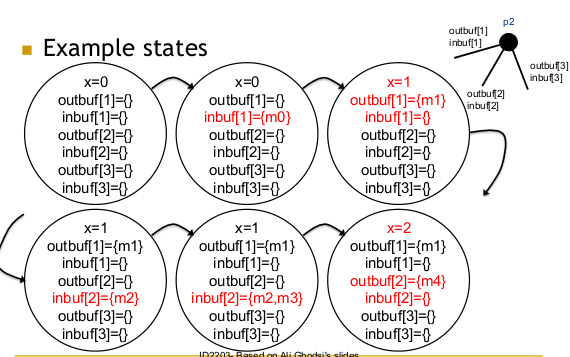
\includegraphics[width=10cm]{img/node.png}
    \caption{Example states}
\end{figure}
\FloatBarrier{}

\paragraph{Working}
\begin{enumerate}
    \item Wait for message
    \item When receive message, do some computation and send message
    \item Goto 1.
\end{enumerate}

\paragraph{Events}
\begin{itemize}
    \item $comp(i)$: computation event at process $i$.
        \subitem{} \textit{Apply transition function $f$ on node $i$ state}
    \item $del(i, j, m)$: delivery event of msg $m$ from $i$ to $j$
        \subitem{} \textit{Move $m$ from outbuf of $p_i$ to inbuf $p_j$}
\end{itemize}

\subsubsection{Transition functions}

Formally a transaction functions requires for any two
$f(<I_1,O_1,s_f1>)=<I_2,O_2,s_2>$ and $f(<I_3,O_3,s_3>)=<I_4,O_4,s_4>$
\begin{itemize}
	\item $I_2=I_4 =<\emptyset,\ldots,\emptyset>$ (all inbufs are empty)
	\item if $I_2=I_4$ and $s_1=s_3$ then
	\begin{itemize}
		\item $s_2=s_4$ (don't observe channel)
		\item $O_1[i] \subseteq O_2[i]$ and $O_3[i] \subseteq O_4[i]$
		(only add msg to outbuf)
		\item $O_2[i]-O_1[i] = O_4[i]-O_3[i]$ (don't observe channel)
	\end{itemize}
\end{itemize}


\subsubsection{Execution}
An execution is a infinite sequence of \enquote{$config_0, event_1, config_1,
event_2, config_2,\cdots$}


\begin{itemize}
    \item[If] $event_k = comp(i)$: $config_{k-1}$ change to $config_k$
        by applying $p_i$'s transition function on i's state in
        $config_{k-1}$
    \item[If] $event_k = del(i, j, m)$: $config_{k-1}$ change to $config_k$
        by moving m from i's outbuf to j's inbuf
\end{itemize}


\subsubsection{Property}

\begin{itemize}
    \item For each $comp(i)$ is associated a \textbf{transition} $(state_1, state_2, i)$
    \item Transition $(s_1, s_2, j)$ is \textbf{applicable} in
        configuration $c$ if accessible state of node $j$ in $c$ is $s_1$
    \item $del(i, j, m)$ \textbf{application} in configuration $c$ if $m$ is
        in outbuf for link $i \leftrightarrow j$ of node $i$ in $c$

        %TODO EXAMPLE SLIDE 11?

    \item \begin{enumerate}
            \item if transition $e=(s_1, s_2, i)$ is applicable
            \item or if $e=del(i, j, m)$ is applicable
        \end{enumerate}
        to configuration $c$, then $app(e,c)$ is the new configuration after
        the event $comp(i)$ or $del(i,j,m)$

\end{itemize}


\subsection{Asynchronous (Schedules) / Synchronous}
Processes are deterministic,
Non-determinism comes from asynchrony (messages take arbitrary time to
be delivered, and the time to compute varies)\ldots \newline

A \textbf{schedule} is the sequence of events. The event are the
one that determine the properties $(del(i,j,m)$ determines the message
asynchrony and $comp(i)$ determines the proccess speed.)
 so all non-determinism is embedded in schedule.

\begin{itemize}
	 \item Given the initial conf, the schedule determines the whole
	 execution.
	 \item Not all schedules are allowed for initial conf. (some
	 event may be impossible to occurs)
\end{itemize}

\subsection{Order of event}
The order in which two applicable computation events or
two applicable delivery events are executed is irrelevant!\\
The idea of the proof is that if you two differents comp
events $a$ and $b$ (meaning on different node!) applicable in a
configuration then appliying $a$ first will not change the state of the
node related to $b$ (vice-versa).
\paragraph{Note} It is only true for event that are not causally
related!
\subsection{Admissible execution (Fairness)}
An execution is admissible if:
\begin{itemize}
	\item Each process has infinite number of $comp(i)$;
	\item Every message m sent is eventually $del(i,j,m)$.
\end{itemize}
The infinity property permit messages to wait arbitrary long times before
being delivered.
\subsection{Synchronous Systems}
The execution is partitionned into disjoint rounds. A round consists of
deliver event for all messages in outbuf and one compute event on
every process.

\subsubsection{Causal order $<_H$}
Causal order is \textbf{transitive}.

\begin{itemize}
    \item[$ a <_H b $]
    \item if $a$ occurs before $b$ on the same process
    \item if $a$ produces $m$ and $b$ delivers $m$
    \item if $a$ delivers $m$ and $b$ consumes $m$
\end{itemize}

\paragraph{Concurrent}
$a$ and $b$ are concurrent (denoted $a || b$), if not $a <_H b$ and not $b <_H a$

\subsection{Similarity of execution}
\begin{itemize}
	\item The view of $p_i$ in $E$, denoted $E|p_i$ is the subsequence
	of executions E restricted to events and state $p_i$.
	\item 2 executions E,F are similar w.r.r if E|$p_i$ = F|$p_i$.
\end{itemize}
\paragraph{Computation Theorem}
\begin{itemize}
	\item Let $E$ an execution ($c_0,e_1,c_1,e_2,\ldots$) and V the
	schedule of event ($e_1,e_2,e_3,\ldots$) s.t. $app(e_i,e_{i-1})=c_i$
	\item Let $P$ be a permutation of V preserving casual order.
\end{itemize}
Then E is similar to the execution starting in $c_0$ with schedule P.
\subparagraph{Notations}
similar execution of E,F is noted F\textasciitilde{} E.
\begin{description}
	\item[Computations or Equivalence class:] A class s.t all the elements
are similar to each other.
\end{description}
Computation theorem implies two importants results:
\begin{enumerate}
	\item There is no algorithm that can observe the order of the sequence
	of events for all executions. %TODO ADD PROOF (pas compris)
	\item Computation theorem does not hold in a model extended s.t each
	process read an hardware clock.%%TODO ADD PROOF (pas compris)
\end{enumerate}
\subsection{Clock}
A clock is used to tell locally if two events are causally related.

\subsubsection{Lamport Clock}
\begin{itemize}
    \item Each process has a local logical clock, $t$ initially $t=0$.
        Node $p$ piggyback $(t, p)$ on every sent message.
    \item On each event:
    \begin{enumerate}
        \item $t = \max(t, t_q) + 1$: when $p$ receives message with
            timestamp ($t_q, q$) (delivery from $q$)
        \item $t = t+1$: for every transistion (comp)
    \end{enumerate}

    \item[$\to$]
        \begin{itemize}
            \item $(t_p, q) < (t_q, q)$ IFF $(t_p <t_q \vee (t_p = t_q \wedge p <
        q))$
\end{itemize}
\end{itemize}

Lamport logical clock guarantee that if $a <_H b$, then $t(a) < t(b)$

\subsubsection{Vector clock}
\begin{itemize}
    \item Each process has a local vector, $v_p$ of size $n$. Initially
        $\forall i : v_p[i]=0$

        Node $p$ piggyback $v_p$ on every sent message.
    \item On each event:
    \begin{enumerate}
        \item $v_p[p] = v_p[p] + 1$
        \item $\forall_i : v_p[i] = \max(v_p[i], v_q[i])$
    \end{enumerate}

\item[$\to$] \begin{itemize}
        \item $v_p \leq v_q$ iff $\forall_i : v_p[i] \leq v_q[i]$
        \item $v_p < v_q$ iff $v_p \leq v_q$ and $\exists i : v_p[i] <
            v_q[i]$
        \item $v_p$ and $v_q$ are concurrent (denoted $v_p \mid\mid v_q$) iff
        $\lnot(v_p < v_q) \land \lnot(v_q < v_p)$
    \end{itemize}
\end{itemize}

Vector clock guarantee that if $v(a) < v(b)$ then $a <_H b$ but also if
$a <_H b$ then $v(a) < v(b)$

\subparagraph{Precisions}
Vector clock cannot be done with smaller vector than size $n$ for $n$ nodes
\begin{itemize}
	\item The relation $<_H$ is a partial order (no ordering of concurrent events)
	\item The relation $<$ on Lamport logical clock is a total order (ordering of clock values)
	\item The relation $<$ on vector timestamps is a partial order (no ordering on TS of concurrent events)
\end{itemize}

\subsection{Complexity}
Defined over the
\begin{itemize}
	\item Number of messages used before terminating
	\item Time it takes to terminate
\end{itemize}
An algorithm has terminated when all states in a config. are terminated
states and there is no more messages in (in/out)bufs.\\
\paragraph{Time Complexity}
A message delay is at most 1 time unit while a computation events take
0 time units. A \textbf{timed execution} is an execution s.t
\begin{itemize}
	\item Time is associated with each $comp(i)$ event
	\item First event happens at time $0$
	\item Time can never decrease and strictly increases locally.
	\item Max time between $comp(i)$ sending $m$ and $comp(j)$
	consuming $m$ is $1$ time unit.
\end{itemize}
Time complexity is maximum time until termination for all
admissible timed executions.


\section{Specification and implementation of distributed systems}

\subsection{Event based component model}
Each node models a sequential program. There is a global clock
and at each tick either a node takes a one of the following step
\begin{itemize}
	\item Computation step: Perfoms computation (local) or
	sends/receives one message to/from other nodes (global)
	\item Communication step: deliver a message.
\end{itemize}
There are different models for the delivery:
\begin{enumerate}
    \item Receive 1 msg and send 1 msg (Guerraoui)
    \item At most receive 1 msg and send at most 1 msg to each neighbor (Lynch)
    \item Receive k msg and send at most 1 msg to each neighbor (Welch)
\end{enumerate}


\paragraph{ }
Each program consists of a set of \textbf{modules or component
specifications}

We study 2 main kinds of distributed systems: \textbf{communications} and
\textbf{reliable high-level services}.

\begin{table}[!ht]
    \begin{tabular}{p{0.475\linewidth}p{0.475\linewidth}}
        \toprule
        \multicolumn{1}{c}{\bf Communication} & \multicolumn{1}{c}{\bf Reliable high-level services} \\
        \toprule
        \begin{itemize}
            \item reliable broadcast
            \item causal order broadcast
            \item total order broadcast
            \item terminating reliable broadcast
        \end{itemize}
        &
        \begin{itemize}
            \item shared memory
            \item consensus
            \item atomic commit
            \item group membership
        \end{itemize} \\
        \bottomrule
    \end{tabular}
\end{table}
\FloatBarrier{}

\subsubsection{Event}
\begin{lstlisting}[mathescape]
upon event <RequestEvent, attr$_1$, attr$_2$,...> do
    // local computation
    trigger <ResponseEvent, attr$_3$, attr$_4$,...>
\end{lstlisting}

There are three main types of event: \textbf{request, indication,
confirmation}

\subsubsection{Modules}

\begin{figure}[!ht]
    \centering
    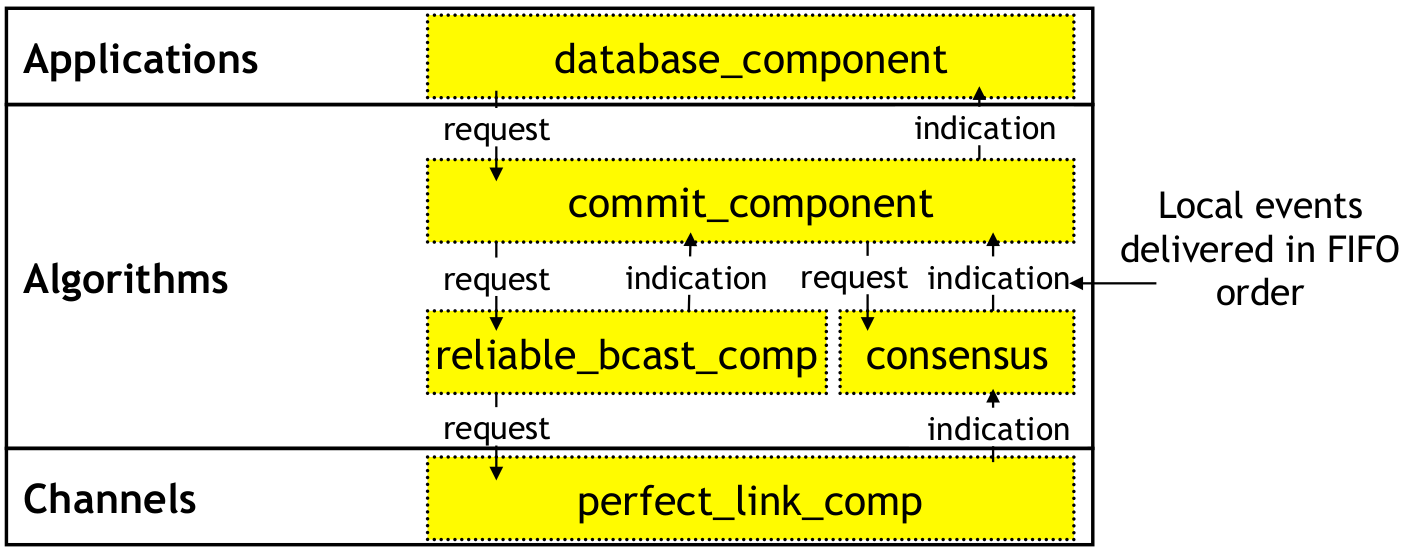
\includegraphics[width=0.6\linewidth]{img/module.png}
    \caption{Modules scheme}
\end{figure}
\FloatBarrier{}

\begin{itemize}
    \item receive instruction:  upon event $<delBcast\ |\ src, [data_1,
        data_2,\ldots] >$ do
    \item send instruction:
        trigger $<sendBcast\ |\ dest, [data_1, data_2,\ldots]>$
\end{itemize}

\begin{figure}[!ht]
    \centering
    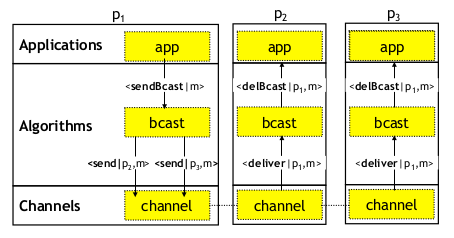
\includegraphics[width=10cm]{img/ex_broadcast.png}
    \caption{Example application uses a broadcast}
\end{figure}
\FloatBarrier{}

\subsection{Specification of a service}

Reliable applications need underlying services strong than network protocols
(such as TCP that only provides a one-to-one connection).

\begin{figure}[!ht]
    \begin{tabular}{m{0.475\linewidth}m{0.475\linewidth}}
        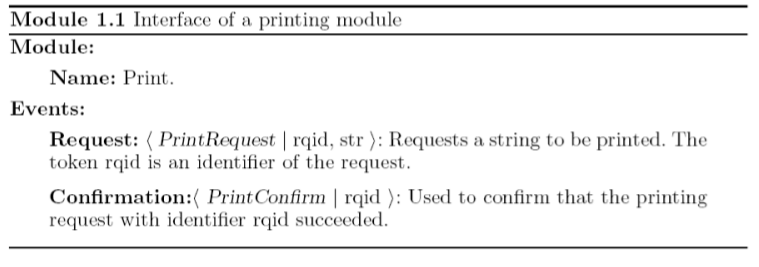
\includegraphics[width=\linewidth]{img/ex_inter1.png} &
        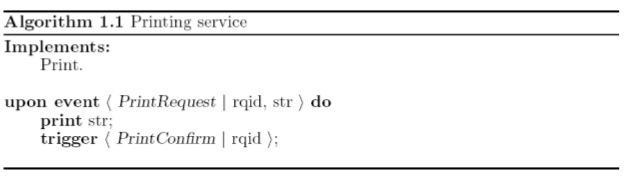
\includegraphics[width=\linewidth]{img/ex_inter2.png} \\
        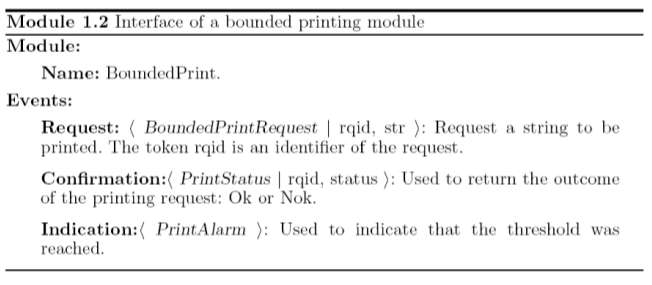
\includegraphics[width=\linewidth]{img/ex_inter3.png} &
        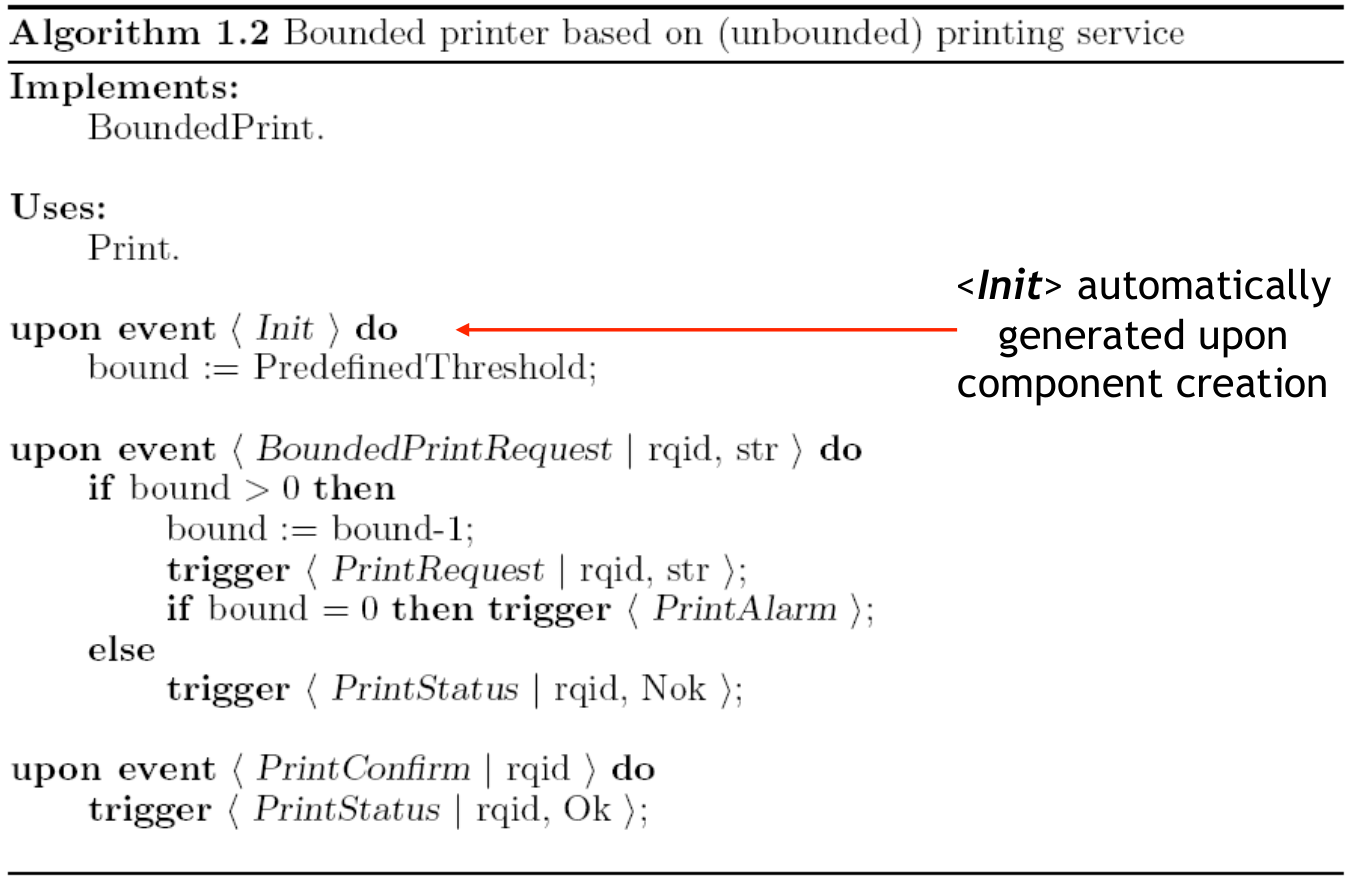
\includegraphics[width=\linewidth]{img/ex_inter4.png}
    \end{tabular}
    \caption{Interface example}
\end{figure}
\FloatBarrier{}


\subsection{Property}

A property P is a function that takes an execution and returns
true/false. (\textit{P is a predicate})

\begin{center}
    \enquote{\textit{Any [property] can be expressed as the conjunction of a
    safety property and a liveness property}}
\end{center}

\begin{itemize}
    \item \textbf{Prefix} of an execution $E$ is the first $k$ (for
        some $k>0$) configurations and events of $E$
    \item \textbf{Extension} of a prefix $P$ is any execution
        that has $P$ as a prefix

    \item \textbf{Safety}: Properties that state that something bad \textcolor{red}{never}
        happens

        \begin{figure}[!ht]
            \centering
            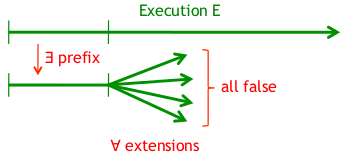
\includegraphics[width=6cm]{img/safety.png}
            \caption{Safety is false if}
        \end{figure}
        \FloatBarrier{}

        \begin{itemize}
            \item[Note:] safety can only be satisfied in infinite time and violated in
                finite time
        \end{itemize}

    \item \textbf{Liveness}: Properties that state that something good
        \textcolor{red}{eventually} happens

        \begin{figure}[!ht]
            \centering
            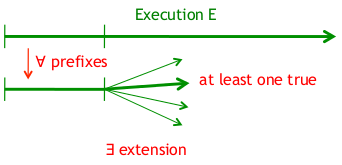
\includegraphics[width=6cm]{img/liveness.png}
            \caption{Liveness is true if}
        \end{figure}
        \FloatBarrier{}

        \begin{itemize}
            \item[Note:] liveness can only be satisfied in finite time and violated in
                infinite time
        \end{itemize}
\end{itemize}


\subsection{Failure}

\subsubsection{Node}

Nodes that don’t fail in an execution are
correct. There are different way of failure:

\begin{itemize}
    \item \textbf{Crash-stop}: stops taking steps, stops sending/receiving msg

        \begin{itemize}
            \item[$\to$] Cannot recover this failure
        \end{itemize}

    \item \textbf{Omissions}: send (resp. receive) ommission. Formally, an
        event removing element from outbuf[i] (resp. inbuf[i])

    \item \textbf{Crash-recovery}: stops taking steps but receiving and
        sending msg.

        \begin{itemize}
            \item[$\to$] We can recover after crashing with special $<Recovery>$ event
                autmatically generated.

                In practice, restarting in initial recovery state or on
                the save state if we make some (expensive) storage on
                permanent storage device.
        \end{itemize}

        A node is faulty in an execution if it crashes and never
        recovers or crashes/recovers infinitely.

        A correct node may crash and recover.

    \item \textbf{Byzantine}: sending messages/updating its state
        not specified by its algorithm.

        \textit{may behave maliciously, attacking the system}

\end{itemize}

\begin{figure}[!ht]
    \begin{tabular}{m{8cm}m{8cm}}
        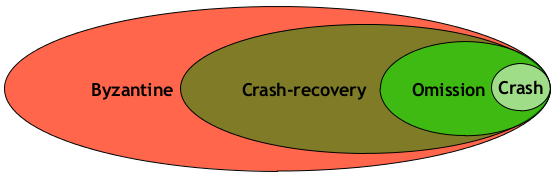
\includegraphics[width=8cm]{img/fault-tolerance.png}
        &
        \begin{itemize}
            \item If node use stable storage: crash-recovery = omission
            \item If node use volatile storage: crash-recovery extend omission
                with amnesia
        \end{itemize}
    \end{tabular}

    \caption{Fault tolerance}
\end{figure}
\FloatBarrier{}

\subsubsection{Channel}

\begin{itemize}
    \item \textbf{Fair-loss links}: Channel delivers any message sent
        with non-zero probability

        \begin{lstlisting}[caption= Fair loss link interface]
Request: <flp2pSend | dest, m>
Indication: <flp2pDeliver | src, m>
        \end{lstlisting}

        \begin{enumerate}
            \item FL1. \textbf{Fair-loss}: If $m$ is sent infinitely
                often by $p_i$
                to $p_j$, and neither crash, then $m$ is delivered infinitely
                often by $p_j$
            \item FL2. \textbf{Finite duplication}: If a $m$ is sent a finite
                number of times by $p_i$ to $p_j$, then it is delivered a
                finite number of times by $p_j$
            \item FL3. \textbf{No creation}: No message is delivered unless it
                was sent
        \end{enumerate}

    \item \textbf{Stubborn links}: Channel delivers any message sent
        infinitely many times (to implement it, we use fair-loss link, each node
        stores the messages sent and periodically resends them).

        \lstinputlisting[caption={Stubborn link interface}, mathescape, captionpos=b]{listings/stubborn_link_interface.erl}

        \begin{enumerate}
            \item[SL1] \textbf{Stubborn delivery}: if a node $p_i$ sends a
                message $m$ to a correct node $p_j$, and $p_i$ does not
                crash, then $p_j$ delivers $m$ an infinite number of
                times

            \item[SL2] \textbf{No creation}: if a message $m$ is delivered by
                some node $p_j$, then $m$ was previously sent by
                some node $p_i$
        \end{enumerate}

    \item \textbf{Perfect links}: Channel that delivers any message
        sent exactly once (keep a set of delivered msg)

        \begin{lstlisting}[caption=Perfect links, mathescape, captionpos=b]
upon event <Init> do
    delivered := $\emptyset$

upon event <pp2pDeliver | dst, m> do
    trigger <sp2pSend | dst, m>

upon event <sp2pDeliver | src, m> do
    if m $\notin$ delivered then
        delivered := delivered $\cup$ {m}
        trigger <pp2pDeliver | src, m>
\end{lstlisting}


        \begin{enumerate}
            \item[PL1] \textbf{Reliable delivery} (liveness):
                If neither $p_i$ nor $p_j$ crashes, then every message sent
                by $p_i$ to $p_j$ is eventually delivered by $p_j$

            \item[PL2] \textbf{No duplication} (safety): Every message is delivered
                at most once

            \item[PL3] \textbf{No creation} (safety): No message is delivered unless it was
                sent
        \end{enumerate}

\end{itemize}

\subsection{Timing assumptions}

Different processing speeds of nodes and different speeds of messages.

\subsubsection{Local vs Global}
\begin{itemize}
    \item Local (one node = State)
        \begin{itemize}
            \item Atomic
            \item Deterministic
        \end{itemize}
    \item Global (many nodes = Configuration)
        \begin{itemize}
            \item Non-atomic (because piece of code in many nodes)
            \item Non deterministic (because of the network and message re-ordering)
        \end{itemize}
\end{itemize}


\subsubsection{Synchronous vs Asynchronous}
\begin{itemize}
    \item Asynchronous: No timing assumption on nodes and channels.

        \begin{itemize}
           \item Lamport clocks (or vector clocks) to observe causality.
           \item Total order not observable
       \end{itemize}

       Internet is asynchronous!

    \item Synchronous: Use round to synchronize (like clock) and this
        is used to detect failure

    \item Partial synchonous: asynchronous system which eventually
        becomes synchronous.

        \textit{It’s just a way to formalize the following: Your
            algorithm will have a long enough time
            window, where everything behaves nicely
        (synchrony), so that it can achieve its goal}
\end{itemize}


\begin{figure}[!ht]
    \centering
    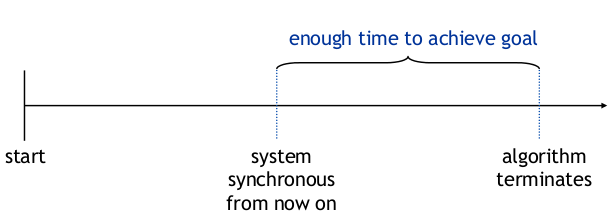
\includegraphics[width=8cm]{img/partialsynchronous.png}
    \caption{Partial synchony}
\end{figure}
\FloatBarrier{}


\section{Failure detectors}

Use failure detectors to encapsulate timing assumptions.
Need completeness and accuracy.

\subsection{Typical implementation}
\begin{enumerate}
    \item Periodically exchange \textbf{heartbeat} messages
    \item Timeout based on worst case RTT
    \item if timeout, then suspect node
    \item if rcv msg from suspected node then revise suspicion and
        increase time-out
\end{enumerate}

\subsection{Modeling}

\begin{itemize}
    \item Configuration = state of each node + \textcolor{red}{FD\_state of each
        node}
    \item Transition function on node $i$ gets extra parameter:
        \textcolor{red}{FD\_state of node $i$}
    \item FD\_state updated in $comp(i)$ by \textcolor{red}{FD\_function}
\end{itemize}

\subsubsection{Requirements}
\begin{itemize}
    \item Completeness (regarding actually crashed nodes)
    \begin{enumerate}
        \item Strong: Every crashed node is eventually detected by \textbf{all}
            correct nodes

            \textit{There exists a time after which all crashed
            nodes are detected by all correct nodes}

        \item Weak: Every crashed node is eventually detected by \textbf{some}
            correct node

            \textit{There exists a time after which all crashed
            nodes are detected by some correct node}
    \end{enumerate}
    \item Accuracy (regarding actually alive nodes)
        \begin{enumerate}
            \item Strong: No correct node is ever suspected

            \item Weak: There exists a correct node which is never
                suspected by any node

            \item Eventual Strong Accuracy: After some finite time the
                FD provides strong accuracy
            \item Eventual Weak Accuracy: After some finite time the FD
                provides weak accuracy
        \end{enumerate}
\end{itemize}

\subsection{Different established detectors}

\begin{table}
    \begin{tabular}{cc|c|c|c}
        \toprule
        & & Strong completeness & Weak completeness & Order\\
        \toprule

        \multirow{2}{*}{Synch} & Strong accuracy & Perfect detector (P) &
        Detector (Q) & (1) \\
        & Weak accuracy & Strong detector (S) & Weak detector (W) & (2) \\

        \midrule

        \multirow{2}{*}{Asyn} & Strong accuracy & Eventually perfect detector
        ($\Diamond P$) & Eventually detector Q ($\Diamond Q$) & (3) \\
        & Weak accuracy & Eventually strong detector ($\Diamond S$) & Eventually weak detector
        ($\Diamond W$) & (4) \\
        \bottomrule
    \end{tabular}
    \caption{$4 \preceq 3, \quad 4 \preceq 2, \quad 2 \preceq 1, \quad 3
    \preceq 1$}
\end{table}

Weak and strong are equivalent. (Weak equivalence $\preceq$ Strong
equivalence is trivial. The inverse is accomplished by a broadcast of
suspected nodes)

\subsubsection{Perfect detector}

There is only one instruction:
\begin{lstlisting}[caption={Perfect failure detector}, mathescape, captionpos=b]
indication <crash | $p_i$>
\end{lstlisting}

There are two properties:

\begin{itemize}
    \item PFD1 \textbf{Strong completeness}: every crashed node is eventually
    detected by \textbf{all} correct nodes
    \item PDF2 \textbf{Strong accuracy}: no correct node is ever suspected
\end{itemize}

\begin{enumerate}
    \item Each node every $\gamma$ time: \texttt{Send <heartbeat>} to all nodes
    \item If don't receive \texttt{<heartbeat>} from node $p_i$ after $\delta + \gamma$ time:
    \texttt{Detect <crash | $p_i$>}
\end{enumerate}

$\Rightarrow$ Synchronous system

\subsubsection{Eventually perfect detector ($\Diamond P$)}:

\begin{lstlisting}[caption={Eventually Perfect detector}, mathescape, captionpos=b]
indication <suspect | $p_i$>
indication <restore | $p_i$>
\end{lstlisting}

\begin{enumerate}
    \item Each node every $\gamma$ time: \texttt{Send <heartbeat>} to all nodes
    \item If don't receive \texttt{<heartbeat>} from node $p_i$ after $T$ time:
    \texttt{Send <suspect | $p_i$>} and add $p_i$ in suspected set
    \item If receive \texttt{<heartbeat>} from node $\in$ suspected:
    \texttt{<restore | $p_i$>} and remove from suspected
\end{enumerate}

$\Rightarrow$ Partially synchronous system


\section{Leader election}

\paragraph{Which node is the leader?}
The lower ID or better the lowest number of crash.

\subsection{Property}
\begin{itemize}
            \item Completeness: eventually every correct node trusts
            some correct node
            \item Accuracy: No two correct nodes trust different correct nodes
        \end{itemize}

\begin{itemize}
    \item Leader election (LE) which matches P
        \begin{itemize}
            \item Eventual completeness: Eventually every correct
            node trusts some correct node. (detects failure)
            \item agreement: No two correct nodes different correct
            nodes.
            \item Local accuracy (if a node is elected leader by $p_i$,
            all previously elected leaders by $p_i$ have crashed)
        \end{itemize}
    \item Eventual leader election (LE) which matches $\Diamond P$
        \begin{itemize}
            \item Eventual completeness (detects failure)
            \item Eventual agreement
        \end{itemize}

\end{itemize}

\subsection{Leader election (LE)}

    \begin{lstlisting}[caption = Leader election with perfect failure detector, mathescape, captionpos=b]
Indication: <leLeader : $p_i$>

upon event <Init> do
    suspected = $\emptyset$
    leader := highest(r)
    trigger <leLeader | leader>

upon event <crash | $p_i$> do
    suspected := suspected $\cup$ {$p_i$}

upon exists $p_i$ s.t. r($p_i$) $\subseteq$ suspected $\wedge$ $p_i \notin$ suspected do
    leader := $p_i$
    trigger <leLeader | $p_i$>
\end{lstlisting}


\begin{enumerate}
    \item[LE1] \textbf{eventual completeness}: Eventually every correct node
    trusts some correct node
    \item[LE2] \textbf{agreement}: no two correct nodes trust different correct
    nodes
    \item[LE3] \textbf{local accuracy}: if a node is elected leader by $p_i$,
    all previously elected leaders by $p_i$ have crashed
    \end{enumerate}

\subsection{Eventual leader election ($\Omega$)}

    \begin{lstlisting}[caption = eventually leader election, mathescape, captionpos=b]
Indication: <leLeader : $p_i$>

upon event <Init> do
    suspected = $\emptyset$
    leader := $p_n$
    trigger <leLeader | leader>

upon event <suspect | $p_i$> do
    suspected := suspected $\cup$ {$p_i$}

upon event <restore | $p_i$> do
    suspected := suspected \ {$p_i$}

upon exists $p_i$ s.t. r($p_i$) $\subseteq$ suspected $\wedge$ $p_i \notin$ suspected do
    leader := $p_i$
    trigger <leLeader | $p_i$>
\end{lstlisting}


\begin{enumerate}
    \item[LE1] \textbf{eventual completeness}: Eventually every correct node
    trusts some correct node
    \item[LE2] \textbf{eventual agreement}: Eventually not two correct nodes trust different correct
    nodes
\end{enumerate}


\subsection{Reductions}
We say $X \preceq Y$ ($X$ is reducible to $Y$) if $X$ can be solved given a
solution of $Y$.

\paragraph{Preorder $\preceq$}:
\begin{itemize}
    \item Reflexivity ($X \preceq X$)
    \item Transitivity ($X \preceq Y \land Y \preceq Z \Rightarrow X \preceq Z$)
\end{itemize}
It is not antisymmetric, thus it's \textbf{not} a partial order.
 We say that $X \simeq Y$ (equivalent) if $X \preceq Y$ and $Y \preceq X$.

\paragraph{Partial order}:
Preorder + antisymmetric

\subsubsection{Trivial reductions}

In the following figures, the arrows ($A \longrightarrow B$) depict the relation
$A \preceq B$.

\begin{figure}[!ht]
    \begin{minipage}{\linewidth}
        \begin{minipage}{0.475\linewidth}
            \centering
            \begin{tikzpicture}[on grid, auto]
                \node (P) {P};
                \node[below left =1cm and 1cm of P] (evP) {$\Diamond P$};
                \node[below right =1cm and 1cm of P] (S) {S};
                \node[below = 2cm of P] (evS) {$\Diamond S$};

                \path[-latex] (evS) edge node {} (evP);
                \path[-latex] (evS) edge node {} (S);
                \path[-latex] (evP) edge node {} (P);
                \path[-latex] (S) edge node {} (P);
            \end{tikzpicture}
            \caption{Strongly complete reductions}
        \end{minipage}
        \begin{minipage}{0.475\linewidth}
            \centering
            \begin{tikzpicture}[on grid, auto]
                \node (Q) {Q};
                \node[below left =1cm and 1cm of Q] (evQ) {$\Diamond Q$};
                \node[below right =1cm and 1cm of Q] (W) {W};
                \node[below = 2cm of Q] (evW) {$\Diamond W$};

                \path[-latex] (evW) edge node {} (evQ);
                \path[-latex] (evW) edge node {} (W);
                \path[-latex] (evQ) edge node {} (Q);
                \path[-latex] (W) edge node {} (Q);
            \end{tikzpicture}
            \caption{Weakly complete reductions}
        \end{minipage}
    \end{minipage}
\end{figure}
\FloatBarrier{}

Completeness is irrelevant: $P \simeq Q$, $S \simeq W$,
$\Diamond P \simeq \Diamond Q$, $\Diamond S \simeq \Diamond W$


\section{Reliable broadcast}

\subsection{Best-effort broadcast}

\begin{itemize}
	\item Best-effort-Validity: if $p_i$ and $p_j$ are correct,
	then any broadcast by $p_i$ is eventually delivered by $p_j$
	\item No duplication: No message delivered  more than once
	\item No creation: No message delivered unless broadcast.
\end{itemize}

BeB gives no guarantee if the sender crash.

\begin{lstlisting}[caption={Best-effort broadcast}, mathescape]
upon event <BebBroadcast | m> do
    for all $p \in dst$
        trigger <BebDeliver | src, m>
\end{lstlisting}


Implementation is straightforward, simple loop on all nodes.

\subsection{Reliable Broadcast}
\begin{itemize}
	\item RB1 \textbf{Validity}: If correct $p_i$ broadcasts $m$, $p_i$ itself
    eventually delivers $m$.
	\item RB2=BEB2 \textbf{No duplication}
	\item RB3=BEB3 \textbf{No creation}
	\item RB4 \textbf{Agreement}: if a correct node delivers $m$, then every
    correct node delivers $m$.
\end{itemize}

\subsubsection{Implementation}
\textbf{Using BEB and P}

    \begin{lstlisting}[mathescape, caption= Lazy reliable broadcast, captionpos=b]
upon event <Init> do
    delivered = $\emptyset$
    correct := $\pi$
    forall $p_i \in \pi$ do
        from[$p_i$] := $\emptyset$

upon event <rbBroadcast | m> do
    trigger <bebBroadcast | (DATA, self, m)>

upon event <crash | $p_i$> do
    correct := correct \ {$p_i$}
    forall ($s_m$, m) $\in$ from[$p_i$] do // redistribute anything from failed node
        trigger <bebBroadcast | (DATA, $s_m$, m)>

upon event <bebDeliver | $p_i$, (DATA, $s_m$, m)> do
    if m $\notin$ delivered then        // avoid duplicates
        delivered := delivered $\cup$ {m}
        from[$p_i$] := from[$p_i$] $\cup$ ($s_m, m$) // store for future
        trigger <rbDeliver | $s_m$, m>
        if $p_i \notin$ correct then // redistribute
            trigger <bebBroadcast | (DATA, $s_m$, m)>
\end{lstlisting}


\paragraph{Proof correctness}
If correct $p_j$ delivers msg broadcast by $p_i$
\begin{itemize}
	\item If $p_i$ is correct, BEB ensures correct delivery
	\item If $p_i$ crashes,
		\begin{itemize}
			\item $p_j$ detects this (completeness).
			\item $p_j$ uses BeB to ensure every correct node gets it.
		\end{itemize}
\end{itemize}
If we use a eventually perfect detector, it only affects
performance, not correctness.


\subsection{Eager Reliable Broadcast}
The exists a eager version of reliable broadcast that does not use a
perfect detector. It simply use a BeB broadcast upon receive of a
message.

    \begin{lstlisting}[mathescape, caption= Eager reliable broadcast, captionpos=b]
upon event <Init> do
    delivered := $\emptyset$

upon event <rbBroadcast | m> do
    delivered := delivered $\cup$ {m}
    trigger <rbDeliver  | self, m>
    trigger <bebBroadcast | (DATA, self, m)>

upon event <bebDeliver | $p_i$, (DATA, $s_m$, m)> do
    if m $\notin$ delivered then
        delivered := delivered $\cup$ {m}
        trigger <rbDeliver | $s_m$, m>
        trigger <bebBroadcast | (DATA, $s_m$, m)>
\end{lstlisting}


\subsubsection{Correctness of Eager RB}
if correct $p_j$ delivers message broadcasted by $p_i$,
$p_j$ uses BeB to ensure every correct node gets it.

\subsection{Uniform reliable broadcast (URB)}
In the above version, uniformity is not respected. If a sender
p immediately RB delivers and crashes, only p will have delivered
the message.

To reach uniformity, if a failed node delivers, everyone must deliver.

\begin{itemize}
    \item URB1=RB1
    \item URB2=RB2
    \item URB3=RB3
    \item RB4 \textbf{Uniform agreement}: for any message $m$, if a process
    delivers $m$, then every correct process delivers $m$.
\end{itemize}

\begin{lstlisting}[mathescape, caption={Uniform reliable broadcast}, captionpos=b]
upon event <urbBroadcast | m> do
    pending := pending $\cup$ {(self, m)} // remember sent messages
    trigger <bebBroadcast | (DATA, self, m)>

upon event <bebDeliver | $p_i$, (DATA, $s_m$, m)> do
    ack[m] := ack[m] $\cup$ {$p_i$} // $p_i$ got m
    if ($s_m$, m) $\notin$ pending then // avoid resending
        pending := pending $\cup$ {($s_m$, m)}
        trigger <bebBroadcast | (DATA, $s_m$, m)>

upon exist ($s_m$, m) $\in$ pending s.t canDeliver(m) AND m $\notin$ delivered do
    delivered := delivered $\cup$ {m}
    trigger <urbDeliver | $s_m$, m>

function canDeliver(m):
    return correct $\subseteq$ ack[m]
\end{lstlisting}


The idea is the following, message are pending until all correct
nodes get it. Node that gets the message exchange ack. The
message is deliver once all the nodes acked.

\subsubsection{Correctness}
\begin{itemize}
    \item No creation from BEB
    \item No duplication by using delivered set
\end{itemize}

\paragraph{Lemma} If a correct node $p_i$ bebDelivers $m$, then $p_i$ eventually
urbDelivers $m$.

\paragraph{Proof} Correct node $p_i$ bebBroadcasts $m$ as soon as it gets $m$

\begin{itemize}
    \item by BEB1 every correct node gets $m$ and bebBroadcasts $m$;
    \item $p_i$ gets $bebDeliver(m)$ from every correct node by BEB1;
    \item by completeness of $P$, it will not wait for dead nodes forever.
\end{itemize}

\paragraph{Majority-ACK Uniform Reliable Broadcast} If a majority of nodes
ack $m$, it reaches the agreement. We change $canDeliver(m)$ to return true when
$\mid ack[m] \mid > n/2$


\section{Causal-Order Broadcast}
Uniform reliable broadcast doesn't deal with the order in which the
message are deliver. The causal-order broadcast remedy to this
problem.

\paragraph{}
We have the relation $m_1 \to m_2$ ($m_1$ causally precedes $m_2$) if
\begin{itemize}
    \item FIFO order: Some process $p_i$ broadcasts $m_1$ before
        broadcasting $m_2$
    \item Network order: Some process $p_i$ delivers $m_1$ and
        later broadcasts $m_2$
    \item Transitivity: There is a message $m'$ s.t $m_1 \to m' \ and \ m'\to m_2$
\end{itemize}
\paragraph{Property}
\begin{itemize}
    \item \textbf{CB:} If node $p_i$ delivers $m_1$, then $p_i$ must have
        delivered every message causally preceding ($\to$) $m_1$ before $m_1$.
    \item \textbf{CB':} If $p_j$ delivers $m_1$ and $m_2$, and $m_1\to m_2$
        then $p_j$ must deliver $m_1$ berfore $m_2$.
\end{itemize}

\begin{figure}[!ht]
    \centering
    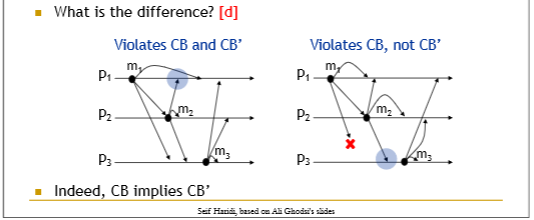
\includegraphics[scale=0.8]{img/cbs_properties.png}
\end{figure}
\FloatBarrier{}

\subsection{Implementation}
The idea is to broadcast the message along with its history (message
that were sent before it). This history is an ordered list of
causally preceding messages called $past_m$

\begin{lstlisting}[caption={Fail-Silent Reliable Causal Order broadcast}, mathescape, captionpos=b]
upon event <Init> do
    delivered := $\emptyset$
    past := nil

upon event <rcoBroadcast | m> do
    trigger <rbBroadcast | (DATA, past, m)>
    past := append(past, <$p_i$, m>)

upon event <rbDeliver | $p_i$, (DATA, past$_m$, m)> do
    if m $\notin$ delivered then
        forall ($s_n$, n) $\in$ $past_m$ do                         // in ascending order
            if n $\notin$ delivered then
                trigger <rcoDeliver | $s_n$, n>        // deliver preceding messages
                delivered := devilered $\cup$ {n}
                past := append(past, <$s_n$, n>) // append to history
        trigger <rcoDeliver | $p_i$, m>               // deliver current message
        delivered := delivered $\cup$ {m}
        past := append(past, <$p_i$, m>)              // append to history
\end{lstlisting}


\subsubsection{First algorithm}
The problem with this algorithm is that the size of the message
grows. The idea to improve the algorithm is to detect with
ack when all correct nodes got the message and delete from
past if it's the case (Garbage Collector). \newline

This algorithm is bad because the $ack[m]$ array also grows with time and the
garbage collector can't work with a $\Diamond P$.

\begin{lstlisting}[caption={Garbage Collected Causal Order Broadcast}, mathescape]
upon event <Init> do
    delivered := $\emptyset$
    past := nil
    correct := $\Pi$
    forall m:
        ack[m] := $\emptyset$  // bookkeeping of acks

upon event <crash | $p_i$> do
    correct := correct \ {$p_i$}

upon event m $\in$ delivered AND seld $\notin$ ack[m] do // called upon coDeliver
    ack := ack[m] $\cup$ {self}
    trigger <rbBroadcast | (ACK, m)>  // ack to all

upon event <rbDeliver | $p_i$, [ACK, m]> do
    ack := ack[m] $\cup$ {$p_i$}
    if correct $\subseteq$ ack[m] do
        past := remove(past, <x, m>)  // When received ack from all, GC m from any x
\end{lstlisting}


%TODO Question on GC

\subsubsection{Second algorithm}
In the first algorithm, the history was a list, in this one it's a
\textbf{vector timestamp} (vector clock). \newline
Each node has a vector clock s.t a node $p_i$:
\begin{itemize}
    \item VC[i]: number of messages $p_i$ coBroadcasted
    \item VC[j], $j \neq i$: number of messages $p_i$ coDelivered from $p_j$
\end{itemize}
The delivery of $m$ is only done if $VC_m$ (attached VC) precedes $VC_i$
(local clock)

\begin{lstlisting}[caption={Vector Clock Causal Order broadcast}, mathescape]
upon event <Init> do
    forall $p_i \in \Pi$ do
        VC[i] := 0

upon event <rcoBroadcast | m> do
    trigger <rbBroadcast | (DATA, VC, m)> // send m with VC
    VC[self] := VC[self] + 1
    trigger <rcoDeliver | self, m> // VC has only increased, so RCO deliver

upon event <rbDeliver | $p_j$, (DATA, VC$_m$, m)> do
    if $p_i \neq$ self then
        pending := pending $\cup$ ($p_j$, (DATA, VC$_m$, m)) // put on hold
        delivered-pending()

procedure delivered-pending()
    while exists x=($s_m$, (DATA, VC$_m$, m)) $\in$ pending s.t VC $\ge$ VC$_m$ do
        pending := pending \ ($s_m$, (DATA, VC$_m$, m)) // remove on hold deliver
        trigger <rcoDeliver | $s_m$, m>
        VC[rank($s_m$)] := VC[rank($s_m$)] + 1 // increase local VC
\end{lstlisting}


\subsection{Different Possible Orderings}
\subsubsection{FIFO order}
\begin{itemize}
    \item Message form same node delivered in order sent.
    \item For all messages $m_1$ and $m_2$ and all $p_i$ and $p_j$:
        \begin{itemize}
            \item if $p_i$ broadcasts $m_1$ before $m_2$, and
                if $p_j$ delivers $m_1$ and $m_2$, then $p_j$ delivers
                $m_1$ before $m_2$.
        \end{itemize}
\end{itemize}

\paragraph{Warning} This definition doesn't require the delivery if both messages.

\subsubsection{Total order}
\begin{itemize}
    \item Everyone delivers everything in exact same order.
    \item For all messages $m_1$ and $m_2$ and all $p_i$ and $p_j$:
        \begin{itemize}
            \item if both $p_i$ and $p_j$ delivers both messages,
                then they deliver them in the same order.
        \end{itemize}
\end{itemize}

\paragraph{Warning} The order is not necessarily the sent order and it does not
require the delivery of both messages

\subsubsection{Hierarchy of Orderings}

Strong \textbf{implies} weaker ordering ($\longrightarrow$)

\begin{figure}[!ht]
    \centering
    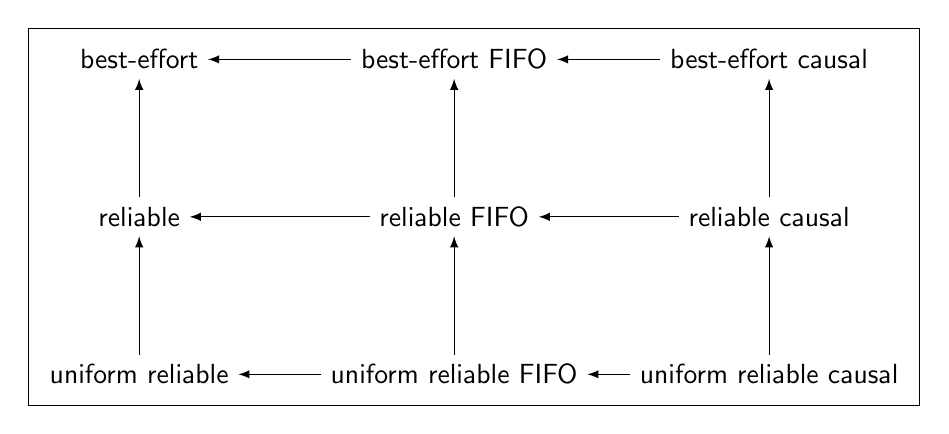
\begin{tikzpicture}[on grid, auto, framed]
        \node (BE) {best-effort};
        \node[right = 4cm of BE] (BEFIFO) {best-effort FIFO};
        \node[right = 4cm of BEFIFO] (BEcausal) {best-effort causal};
        \node[below = 2cm of BE] (reliable) {reliable};
        \node[below = 2cm of BEFIFO] (reliableFIFO) {reliable FIFO};
        \node[below = 2cm of BEcausal] (reliablecausal) {reliable causal};
        \node[below = 2cm of reliable] (uniformreliable) {uniform reliable};
        \node[below = 2cm of reliableFIFO] (uniformreliableFIFO) {uniform reliable FIFO};
        \node[below = 2cm of reliablecausal] (uniformreliablecausal) {uniform reliable causal};

        \path[-latex] (uniformreliablecausal) edge node {} (uniformreliableFIFO);
        \path[-latex] (uniformreliableFIFO) edge node {} (uniformreliable);
        \path[-latex] (uniformreliablecausal) edge node {} (reliablecausal);
        \path[-latex] (reliable) edge node {} (BE);
        \path[-latex] (reliableFIFO) edge node {} (BEFIFO);
        \path[-latex] (reliablecausal) edge node {} (BEcausal);
        \path[-latex] (BEcausal) edge node {} (BEFIFO);
        \path[-latex] (BEFIFO) edge node {} (BE);
        \path[-latex] (uniformreliable) edge node {} (reliable);
        \path[-latex] (uniformreliableFIFO) edge node {} (reliableFIFO);
        \path[-latex] (reliablecausal) edge node {} (reliableFIFO);
        \path[-latex] (reliableFIFO) edge node {} (reliable);
    \end{tikzpicture}
    \caption{Hierarchy of Orderings}
\end{figure}
\FloatBarrier{}


\section{Shared Memory}

In real shared memory there is no message-passing, node access one
shared memory. But in distributed system we simulate shared memory
using message passing.

\begin{itemize}
	\item A register represents each memory location (objects)
    \item Node can \texttt{read(R) => x}/\texttt{write(R, x)}
	\item Simplification of key-value stores
\end{itemize}

\paragraph{Basic Assumptions}
\begin{itemize}
    \item Nodes are sequential, they can only do one operation at a time.
invocation,response,invocation,response,\ldots
\item The values are positive integers initially zero.
    \end{itemize}

\paragraph{Definitions}
In an execution, an operation is
\begin{itemize}
	\item \textbf{complete} if both invocation \& response occured
	\item \textbf{failed} if invoked, but no response arrives
\end{itemize}

$op_1$ precedes $op_2$ if (denoted $<_p$) if response of $op_1$
precedes invocation of $op_2$. Otherwise they are concurrent.

\paragraph{Terminology}
\begin{itemize}
	\item (1,N)-algorithm: 1 designated writer, multiple readers
	\item (N,N)-algorithm: Multiple writers, multiple readers
\end{itemize}


\subsection{Regular Register (1,N)}
\begin{itemize}
	\item Termination: Each read and write operation of a correct node
	completes.
	\item Validity: Read return last value written if
		\begin{itemize}
			\item Read is not concurrent with another write, and
			\item Read is not concurrent with a failed operation
		\end{itemize}
	Otherwise the read must return the last value
	written or a concurrent value being written.
\end{itemize}


\subsubsection{Centralized Algorithm}

One process is designated as leader. For reading, the latest value must
be asked to the leader. For writing, leader's value is updated.

$\Rightarrow$ does not work if leader crashes.

\subsubsection{Bogus Algorithm}
\begin{itemize}
    \item[read]: return local value
    \item[write]: overwrite local value and broadcast change
\end{itemize}

\begin{figure}[!ht]
    \centering
        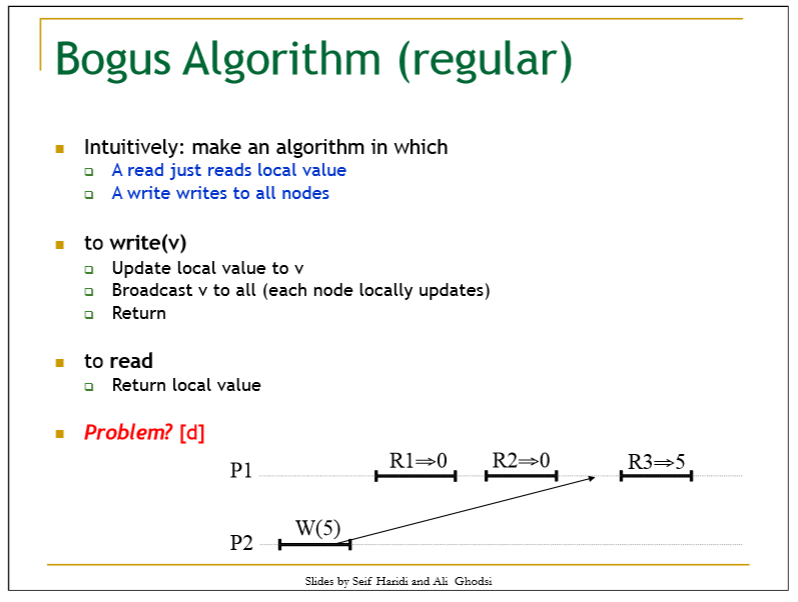
\includegraphics[width=6cm]{img/bogus_1.png}
        \caption{Bogus algorithm}
\end{figure}
\FloatBarrier{}

\paragraph{Read-one write all (1, N)}
Bogus algorithm modified can be use with a \textbf{perfect FD}
and fail-stop model.

\begin{itemize}
    \item[$\to$] write needs to wait \enquote{ACK} from all correct nodes when he
    broadcasts updated local value.
    \item[$\to$] read returns local value.
\end{itemize}

\subsubsection{Majority Voting Algorithm}
Main idea is based on a quorum principle,
\begin{itemize}
	\item Always write to and read from a majority of nodes
	\item At least one node knows most recent value
\end{itemize}

\paragraph{Quorum Principle}
Divide the system into quorums, any two quorums should intersect.
There are different type of quorum
\begin{itemize}
	\item Majority Quorum
		\begin{itemize}
            \item[Pro]: tolerate up to $\lceil N/2 \rceil -1$ crashes
            \item[Con]: Have to read/write $\lfloor N/2 \rfloor + 1$ values
		\end{itemize}
	\item Maekawa Quorum
		\begin{itemize}
			\item Arrange nodes in $M \times M$ grid ($M=sqrt(N)$)
			\item Write to rows, read to columns (always overlap)
            \item[Pro]: Only need to read/write $sqrt(N)$ nodes
            \item[Con]: Tolerate at most $sqrt(N)-1$ crashes
		\end{itemize}
\end{itemize}

\paragraph{Implementation}

\begin{table}[!ht]
    \begin{tabular}{>{\centering}m{0.2\linewidth}|m{0.7\linewidth}}
        \hline
        $read$ & \begin{enumerate}
                \item Broadcast read request
                    \begin{itemize}
                        \item[$\to$] receiver response with local value and seq\#
                    \end{itemize}
                \item Save values from majority of nodes
                \item Return value with highest seq\#
            \end{enumerate} \\
        \hline
        $write(v)$ & \begin{enumerate}
            \item Broadcast $v$ and seq\#
                \begin{itemize}
                    \item[$\to$] receiver update to $v$ \textcolor{red}{if newer seq\#}
                \end{itemize}
            \item Wait for ACK from majority of node then increments seq\#
        \end{enumerate} \\ \hline
    \end{tabular}
    \caption{Implementation of Majority Voting Algorithm (1,N)}
\end{table}
\FloatBarrier{}

The problem with the basic algorithm is that old write can overwrite
new write. (resolved by the added \textcolor{red}{red part})

\subsection{Single Storage}

\paragraph{Safety requirements}
\begin{itemize}
	\item \textbf{Sequential Consistency}: Only allow executions whose results
	appear as if there is a single system image and \enquote{local time} is
	obeyed
	\item \textbf{Linearizability/Atomicity}: Only allow executions whose
	results appear as if there is a single system image and
	\enquote{global time} is obeyed.
\end{itemize}

\paragraph{Liveness: progress\newline}

Liveness requirements: three progressively weaker versions
\begin{itemize}
	\item \textbf{Wait-free} (strongest): Every correct node should \enquote{make progress}
	(no deadkocks, no livelocks, no starvation)
	\item \textbf{Lock-free/non-blocking}: At least one correct node should
	\enquote{make progress} (no deadlocks, no livelock, maybe starvation)
	\item \textbf{Obstruction free/solo-termination}: If a single node executes
	without interference (contention) it makes progress
	(no deadlocks, maybe livelocks, maybe starvation)
\end{itemize}

\subsection{Atomic/Linearizable Registers}

\begin{itemize}
	\item Termination (Wait-freedom): If a node is correct, each read and write op
	eventually completes
	\item Linearization Points:
	\begin{itemize}
		\item \textbf{Read ops} appears as if immediately happened at all nodes
		at some time between invocation and response.
		\item \textbf{Write ops} appears as if immediately happened at all nodes
		at some time between invocation and response.
		\item \textbf{Failed ops} appears as whether completed at every node
		whether never occured at any node
	\end{itemize}

    \paragraph{Equivalent with}
    \begin{itemize}
        \item Validity: read
            \begin{enumerate}
                \item[IF] read not conurrent with another write or with a failed operation
                    return last value written
                \item[ELSE] return concurrent value written
            \end{enumerate}
        \item Ordering: if read $r_1$ precede read $r_2$ then write $r1$ precedes $r2$
    \end{itemize}
\end{itemize}

\paragraph{Majority voting}
There is a problem with the majority voting as the system could appear
as non atomic.

\subsubsection{Atomic register: Single writer (1,N))}

Solution to previous issues: when reading, also make a write before responding.

$\Rightarrow$ Use \textbf{causality} to enforce \textbf{atomicity}.

\begin{figure}[!ht]
    \centering
    \begin{tabular}{m{7cm}m{7cm}}
		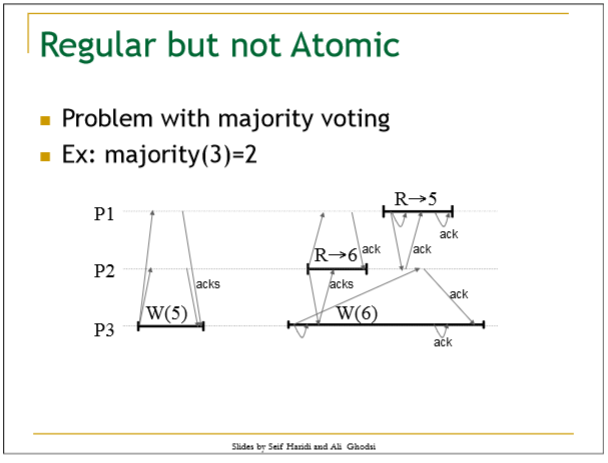
\includegraphics[width=7cm]{img/maj_prob.png}&
		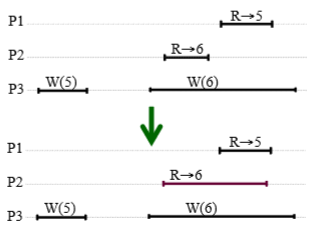
\includegraphics[width=6cm]{img/maj_sol.png}
	\end{tabular}
		\caption{Majority Voting Problem and Solution}
\end{figure}
\FloatBarrier{}

\subsubsection{Atomic register: Multiple writers (N,N))}

With multiple writers, their seq\# might be non-synchronized
which has the effect of ignoring some write operations.

\paragraph{Solution}
\begin{enumerate}
	\item Get seq\# before writing by reading from
	the majority (to get last seq\#)
	\item Send Ack if receive write with old \#seq
\end{enumerate}

\paragraph{Message passing}
Message passing can be simulated using shared memory. The idea
consist of using a register AB to simulate the channel between A and B like a pipe.

\begin{itemize}
    \item $\to$ Message passing and shared memory equivalent in functionality
but not in always in efficiency.
\end{itemize}

\subsection{Linearizability}
\subsubsection{Formalism}
\begin{itemize}
	\item $R-inv_i(X)$ Read invocation by node i on register X
	\item $R-res_i(a)$ Response with value a to read by node i
	\item $W-inv_i(X,a)$ Write invocation by node i on register
	X with value a.
	\item $W-res_i$ Response (confirmation) to write by node i
\end{itemize}

\subsubsection{Executions}
Every execution consists of:
\begin{itemize}
	\item Read operations composed of two events:
	$R-inv_i(X)$ and $R-res_i(a)$
	\item Write operations which consist of two events:
	$W-inv_i(X,a)$ and $W-res_i$
	\item An execution is sequential if:
	\begin{itemize}
		\item X-inv by $i$ immediately followed by a corresponding X-res at $i$
		\item X-res by $i$ immediately follows a corresponding X-inv by $i$
		\item no concurrency, read $x$ by $p_1$, write $y$ by $p_5$,\ldots
	\end{itemize}
\end{itemize}

\subsubsection{Assumptions}
\begin{itemize}
    \item An operation $O$ is \textbf{pending} in execution $E$ if $O$ has no
    response event
    \item An execution is \textbf{complete} if every operation is complete
    (else partial)
    \item An operation $X$ \textbf{precedes} operation $Y$ in execution $E$ if
    response of $X$ is before invocation of $Y$ in $E$
    \end{itemize}

\subsubsection{Linearizability formally}

Consider two executions $E$ and $F$.

\begin{table}[!ht]
    \begin{tabular}{p{0.475\linewidth}|p{0.475\linewidth}}
        Linearizability w/o failure (sequential consistency) & Linearizability with failure (partial execution) \\
        \hline
        A complete $E$ is \textbf{linearizable} if $\exists$ F s.t.
        \begin{itemize}
            \item \textbf{Similarity} events(E) = events(F)
            \item \textbf{No concurrency} F is sequential
            \item \textbf{Legal operations}
            \item \textbf{Time ordering} if $X \preceq Y$ in $E$, $X \preceq Y$ in $F$
        \end{itemize} & A partial $E$ is \textbf{linearizable} if $E$ is modified s.t.
        \begin{itemize}
            \item Every pending operation is completed by
            \begin{itemize}
                \item removing the invocation of the operation, or
                \item adding a response to the operation
            \end{itemize}
            \item $F$ is linearizable
        \end{itemize} \\
    \end{tabular}
\end{table}
\FloatBarrier{}


\section{Consensus}

Nodes proposes value and they must agree on one of these values.

\paragraph{Key problem} Solve total order broadcast, atomic commit, reliable broadcast

\subsection{Properties}

\begin{description}
	\item[Validity] Any value decided is a value proposed
	\item[Agreement] No two correct nodes decide differently
	(in a \textbf{uniform consensus}, node does not need to be correct)
	\item[Termination] Every correct node eventually decides
	\item[Integrity] A node decides at most once
\end{description}

\begin{lstlisting}[caption={Consensus interface}]
Request: <cPropose | v>
Indication: <cDecide | v>
\end{lstlisting}


\subsection{Hierachical Consensus}

\begin{itemize}
    \item Use perfect failure detector $P$ and a best-effort broadcast $BEB$
    \item Each node stores its \texttt{proposal} and the identifier of the last
    adopted proposer in \texttt{lastprop}.
    \item Loop through rounds $1$ to $N$
        \begin{tabular}{m{1.3cm}m{13cm}}
            Round $i$ &
        \begin{itemize}
            \item node $i$ is leader and broadcasts and decides its proposal $v$
            \item Other nodes adopt $i$ proposal $v$ (save it in lastprop) or
                detect crash of $i$.
            \item[$\to$] Future rounds will only propose $v$
        \end{itemize}
    \end{tabular}
\end{itemize}

\subsubsection{Orphan message issue}

Problem is that broadcast can be delayed and the leader crash
and a node can receive two proposal in the next round. It will
therefore affect future round.

\begin{figure}[!ht]
    \centering
    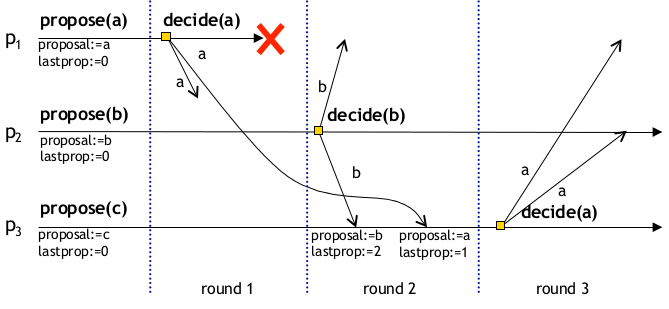
\includegraphics[width=8cm]{img/orphan.png}
    \caption{Orphan}
\end{figure}
\FloatBarrier{}

\paragraph{Solution}

Counter measure $\to$ ranking of the node based on there identifier
($p_1>p_2>p_3>\ldots$)

$\Rightarrow$ Adopt if proposer $p$ is ranked lower than lastprop otherwise $p$ has
crashed and should be ignored

\subsubsection{Implementation}

    \begin{lstlisting}[caption={Hierachical consensus}, mathescape]
upong event <Init> do
    detected :=  $\emptyset$
    round     := 1
    proposal := $\perp$ // last adopted proposal
    lastprop := 0  // last adopted proposer id
    for i=1 to N do
        broadcast[i] := delivered[i] := false

upon event <crash | $p_i$ do
    detected := detected $\cup$ {rank($p_i$)}

upon event <cPropose | v> do
    if proposal = $\perp$ then // set node's initial proposal unless it already has
        proposal := v

upon round = rank(self) and    // if I am leader
     broadcast[round] = false and   // trigger once per round
     proposal != $\top$ do    // trigger if I have proposal

    broadcast[round] := true
    trigger <cDecide | proposal>    // permanently decide
    trigger <bebBroadcast | (DECIDED, round, proposal)>

upon event <bebDeliver | $p_i$, (DECIDED, r, v)> do
    if r > lastprop then // invariant: only adopt newer than what you have
        proposal := v
        lastprop := r
    delivered[r] := true

upon delivered[round] or round $\in$ detected do
    round := round + 1  // next round if deliver or crash
\end{lstlisting}


\subsubsection{Correctness}
\begin{itemize}
	\item Validity? $\to$ Always decide own proposal or adopted value
	\item Integrity? $\to$ Rounds increase monotonically, node only
	decide when leader.
	\item Termination? $\to$ Every correct node makes it to the round it
	is leader in:
	\begin{itemize}
		\item If some leader fails, completeness of $P$ ensure progress.
		\item If leader correct, validity of BEB ensures delivery.
	\end{itemize}
	\item Agreement? $\to$ take correct leader with minimum id $i$.
        \begin{itemize}
            \item By termination it will decide $v$ and $v$ will be BEB
            \item[$\to$] Every correct node adopts $v$ no older proposal
                can override the adoption
        \end{itemize}
\end{itemize}

\textbf{Failure-torerant up to N-1}

\subsubsection{Formalism}
\begin{lstlisting}[caption={Hierarchical consensus}, mathescape]
$x_i$ := proposal
for r:=1 to N do
    if r=i then
        forall j in 1..N do
            send <val, $x_i$, r> to $P_j$;
        decide $x_i$
    if collect <val, x', r> from r then
        $x_i$ := x';
end
\end{lstlisting}

\subsection{Uniform consensus}
To reach uniform consensus, we move the decision to the end.

\begin{lstlisting}[caption={Uniform Hierarchical consensus with P}, mathescape]
$x_i$ := input
for r:=1 to N do
    if r=i then
        forall j in 1..N do
            send <val, $x_i$ , r> to $P_j$;
    if collect <val, x', r> from r then
        $x_i$ := x';
end
decide $x_i$
\end{lstlisting}

\subsubsection{With inaccurate FD}

\begin{figure}[!ht]
    \centering
    \begin{tabular}{m{8cm}m{8cm}}
        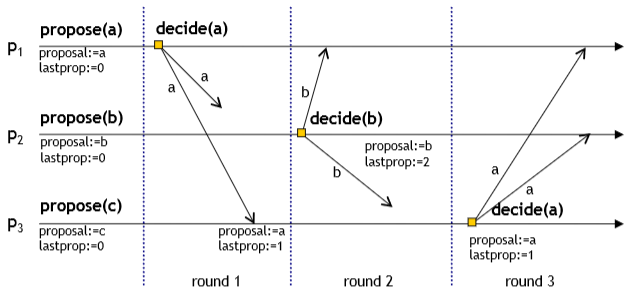
\includegraphics[width=8cm]{img/hc_fd.png} &
        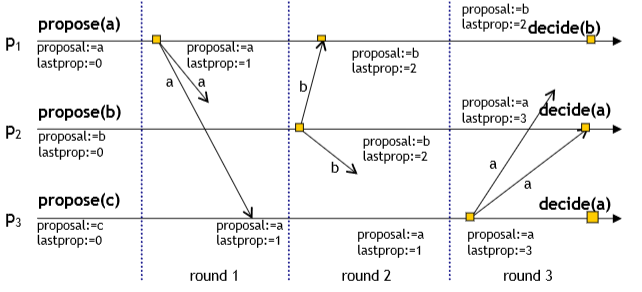
\includegraphics[width=8cm]{img/uhc_fd.png} \\
        p2 suspect p1, p3 suspect p2 (nonuniform consensus) &
        p2 suspect p1, p3 suspect p2, p1 suspect p3 (uniform consensus)\\
        \multicolumn{2}{c}{$\Rightarrow$ Doesn't work with innacurrate FD}
    \end{tabular}
        \caption{Inaccuracy with failure detector}
\end{figure}
\FloatBarrier{}

\textbf{The algorithm doesn't work with inaccurate FD}

\subsubsection{With Strong failure detector}

The algorithm works with a $S$ (strong detector). The difference between
Strong detector (weaker than $P$) and a Perfect detector comes from the
accuracy w.r.t one node.

\paragraph{Correctness}
\begin{itemize}
	\item Validity? $\to$ Always decide own proposal or adopted value
	\item Integrity? $\to$ Rounds increase monotonically, node only
	decides once in the end.
	\item Termination? $\to$ Every correct node makes it to the last round
	\begin{itemize}
		\item If some leader fails, completeness of $S$ ensures progress.
		\item If leader correct, validity of BEB ensures delivery.
	\end{itemize}
	\item Uniform agreement? $\to$ take an accurate correct leader with id $i$.
        \begin{itemize}
            \item By weak accuracy (S) and termination such a node exists
                and it will BEB $v$
        \end{itemize}
\end{itemize}


\subsubsection{With Eventual failure detector}
Eventually perfect detector cannot solve consensus with resilience $t \geq n/2$

%Proof?
\begin{itemize}
	\item Rotating coordinator from before will not work because
	\enquote{eventually} might be after the first $N$ rounds
	\item The idea is to rotate forever and eventually all nodes
	correct w.r.t. 1 coordinator (coordinator's value becomes
	agreed value)
\end{itemize}

\paragraph{Termination}
There will be a bound on the number of failures $\to$ less ($f<n/3$) than a third
can fail. This will allow to decide using majority.

\begin{enumerate}
	\item Everyone send vote to coordinator $C$
	\item $C$ picks majority vote $V$, and broadcasts $V$
	\item Every node get broadcast, change vote to $V$
	\item Change coordinator $C$ and go to 1
\end{enumerate}

\begin{lstlisting}[caption={Rotate coordinator for $\Diamond S$}, mathescape]
$x_i$ := input
r=0
while true do
begin
    r := r + 1
    c := (r mod n) + 1  // rotate to coordinator c
    send <value, $x_i$, r> to $p_c$ // all send value to coord

    if i==c then  // coord only
    begin
        msgs[0]:=0; msgs[1]:=0;    // reset 0 and 1 counter
        for x:=1 to N-f do
        begin
            receive <value, V, R> from q  // receive N-f msgs
            msgs[V]++;       // increase relevant counter
        end
        if msgs[0] > msgs[1] then v := 0 else v := 1 end // choose majority value
        if msgs[0]==0 or msgs[1]==0 then d := 1 else d := 0 end // all N-f same ?
        forall j do send <outcome, v, r> to $p_j$ // send v to all
    end

    if collect<outcome, v, r> from $p_c$ then   // collect value from coord
    begin
        $x_i$ := v  // adopt v
        if d and i!=0 then begin decide(v); i:=0; end
    end
end
\end{lstlisting}

\begin{itemize}
    \item If at least $n-f$ nodes vote $V$ in round $r$, every leader will see
    a majority for $V$ in all rounds > r.

        \paragraph{Proof}:
        \begin{itemize}
            \item We know that at most $f$ nodes don't vote $V$
            \item We also know $n/3<(n-f)/2$ (because $f<n/3$ implies $n-f>2n/3$)
                $\to f<(n-f)/2$ (because $f<n/3$ and $n/3<(n-f)/2$)
            \item So less than half of any $n-f$ nodes do not vote $V$
        \end{itemize}
\end{itemize}


\section{Terminating Reliable Broadcast (TRB)}

With normal reliable broadcast, no idea when or if a message will be delivered.

$\Rightarrow$ In TRB, sender broadcast $M$ and receiver await delivery $M$. All
nodes either deliver $M$ or \enquote{abort} (special sender faulty message <SF>)

TRB requires synchrony!

\begin{lstlisting}
Request: <trbBroadcast | src, m>
Request: <trbBroadcast | src, m>
\end{lstlisting}

\subsection{Property}
\begin{description}
	\item[TRB1. Termination] Every correct node eventually delivers one message
	\item[TRB2. Validity] If correct src sends $m$, then src will deliver $m$
	\item[TRB3. Uniform agreement] If any node delivers $m$, then every correct node
	eventually delivers $m$
	\item[TRB4. Integrity] If a node delivers $m$, then either $m=<SF>$ or $m$ was
	broadcast by src.
\end{description}

\subsection{Consensus based TRB}
Src RB broadcast $m$ (deliver <SF> if src is suspected by $P$)
\begin{itemize}
	\item Src BEB broadcast $m$
	\item Nodes propose whichever comes first: crash suspicion(<SF>) or
	BeB delivery from src (M)
	\item Deliver consensus decision
\end{itemize}


\subsubsection{Hardness}
\begin{itemize}
    \item $consensus \preceq TRB$ $\Rightarrow$ can't implement TRB in asynchronous networks.
    \item $ P \preceq TRB \land TRB \preceq P \Rightarrow TRB \simeq P$: can't
    implement TRB in eventually synchronous systems (with $\Diamond P$)
\end{itemize}

\subsubsection{Correctness}
TODO

\section{Total order broadcast (consensus)}

The order imposed by causal broadcast is partial. Some message might
be delivered in different order by different process.

With \textbf{total order} broadcast, process must deliver all
messages according to the same order.

\paragraph{\textbf{Total order broadcast} $\equiv$ \textbf{consensus}}

\subsection{Specification}
The specification of the total order broadcast are roughly the same as the
reliable broadcast there only a little modification.

\begin{description}
    \item[RB1. Validity] If $p_i$ and $p_j$ are correct, then every message
    broadcast by $p_i$ is eventually delivered by $p_j$
    \item[RB2. No duplication] No message is delivered more than once
    \item[RB3. No creation] No message is delivered unless it was broadcast
	\item[RB4. Uniform agreement] For any message $m$: if any process delivers
	$m$, then every correct process delivers $m$.
\end{description}
\
\subsection{Type of total order}

\begin{lstlisting}
Request: <toBroadcast, m>
Indication: <toDeliver, src, m>
\end{lstlisting}

\subsubsection{Total order}
\begin{itemize}
	\item Let $m_1$ and $m_2$ be any two messages and let $p_i$ and $p_j$ be any
    two correct processes that deliver $m_1$ and $m_2$
	\item If $p_i$ delivers $m_1$ before $m_2$, then $p_j$ delivers $m_1$ before
    $m_2$
\end{itemize}

\subsubsection{Uniform total order}
\begin{itemize}
	\item Let $m_1$ and $m_2$ be any two messages and let $p_i$ and $p_j$ be any
    two processes that deliver $m_2$ (only $m_2$!).
	\item If $p_i$ delivers $m_1$ before $m_2$, then $p_j$ delivers $m_1$ before
    $m_2$
\end{itemize}

\subsubsection{Components of a process (node)}

\begin{figure}[!ht]\centering
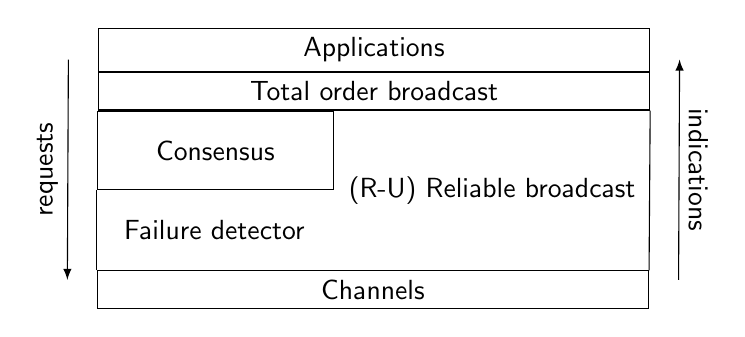
\begin{tikzpicture}
    \node[draw, minimum width = 7cm] (Applications) {Applications};
    \node[draw, below = 0cm of Applications, minimum width=7cm] (TOB) {Total order broadcast};
    \node[draw, below left = 0cm and -3cm of TOB, minimum width=3cm, minimum height=1cm] (Consensus) {Consensus};
    \node[below right = -1cm and 0cm of Consensus, minimum width=4cm, minimum height=2cm] (RB) {(R-U) Reliable broadcast};
    \node[below left = 0cm and -3cm of Consensus, minimum width=3cm, minimum height=1cm] (FD) {Failure detector};
    \node[draw, below right = 0cm and -3cm of FD, minimum width=7cm] (Channels) {Channels};
    \node[left = 0.25cm of Applications] (A) {};
    \node[left = 0.25cm of Channels] (B) {};
    \node[right = 0.25cm of Applications] (C) {};
    \node[right = 0.25cm of Channels] (D) {};
    \draw (Channels.north west) -- (Consensus.south west);
    \draw (Channels.north east) -- (TOB.south east);

    \path[-latex] (A) edge node [rotate=90,above] {requests} (B);
    \path[-latex] (D) edge node [rotate=270,above] {indications} (C);
\end{tikzpicture}
    \caption{Components of a process}
\end{figure}
\FloatBarrier{}

\subsection{Consensus based algorithm}
\begin{lstlisting}[caption=Total order implementation, mathescape]
upon event <Init> do
    unordered = delivered = $\emptyset$
    wait := false
    sn := 1

upon event <toBroadcast, m> do
    trigger <rbBroadcast, m>

upon event <rbDeliver, sm, m> AND (m $\notin$ delivered) do
    unordered := unordered $\cup$ {(sm, m)}

upon (unordored $\neq \emptyset$) AND not(wait) do
    wait := true
    trigger <Propose sn, unordered>

upon event <Decide sn, decided> do
    unordered := unordered \ decided
    ordered := deterministicSort(decided)

    for all (sm, m) $\in$ ordered:
        trigger <toDeliver, sm, m>
        delivered := delivered $\cup$ {m}

    sn := sn + 1
    wait := false
\end{lstlisting}

\paragraph{Equivalences} Therefore, \textbf{consensus} and \textbf{total order
broadcast} are \textbf{equivalent} problems in a system with reliable channels.

\section{Group Membership}

\begin{itemize}
    \item Processes sometimes need to know which processes are participating in
    the computation and which are not.

    \item Failure detectors provide such information but the information isn't
        coordinated even if failure detector is perfect.

        (Crash detected at different time for different processes)
\end{itemize}

\begin{figure}[!ht]
    \centering
    \begin{tabular}{cc}
        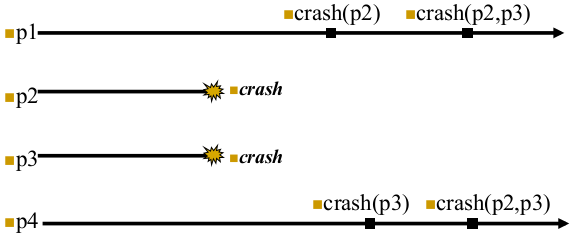
\includegraphics[width=7cm]{img/gm1.png}&
        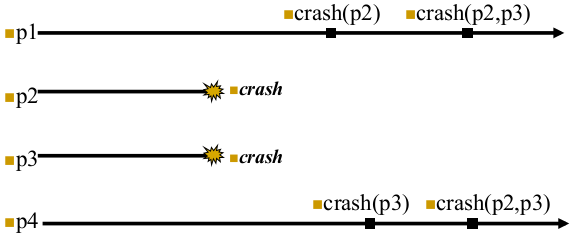
\includegraphics[width=7cm]{img/gm1.png}\\
    \end{tabular}
    \caption{Group membership}
\end{figure}
\FloatBarrier{}

\begin{itemize}
	\item Like FD, processes are informed about failures; we say that
	the processes install \textbf{views}.
	\item Like PFD, processes have accurate knowledge about failures.
	\item Unlike a PFD, the information about failures are
	coordinated, the processes install the same sequence of view.
\end{itemize}

\subsection{Properties (considering only crashes)}
\begin{description}
	\item[Local Monotonicity] If a process install view $(j,M)$ after
        installing $(k,N)$, then $j > k$ and $M \subset N$
	\item[Agreement] No two processes install views $(j,M)$ and $(j,M')$ such that
	$M \neq M'$
	\item[Completeness] If a process $p$ crashes, then there is an integer
	$j$ such that every correct process eventually installs view $(j,M)$ such that
	$p$ is not in $M$
	\item[Accuracy] If some process installs a view $(i,M)$ and $p$ is not in $M$,
	then $p$ has crashed
\end{description}

\subsection{Algorithm}
\begin{lstlisting}[caption=Group membership, mathescape]
upon event <Init> do
    view := (id:0, memb:$\Pi$)
    correct := $\Pi$
    wait := false

upon event <crash $p_i$> do
    correct := correct \ {$p_i$}

upon event (correct $\subset$ view.memb) and (wait == false) do
    wait := true
    trigger <ucPropose (view.id + 1, correct)>

upon event <ucDecided (i, m)> do
    view := (id:i, memb:m)
    wait := false
    trigger <membView view>
\end{lstlisting}

\begin{figure}[!ht]
		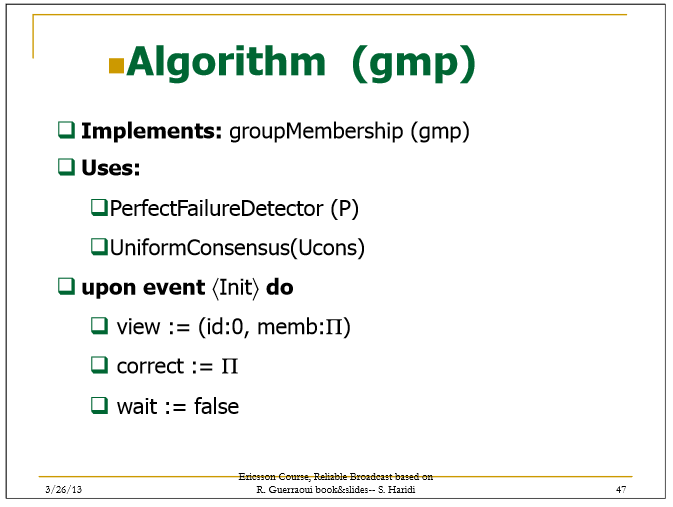
\includegraphics[width=8cm]{img/gmp_1.png}
	\caption{Group membership}
\end{figure}
\FloatBarrier{}

\subsection{Non-blocking atomic commit}
\begin{lstlisting}
Request: <nbacPropose | v>      // propose value for the commit (0 or 1)
Indication: <nbacDecide | v>    // indicate decided value
\end{lstlisting}

\begin{itemize}
    \item[NBAC1]: \textbf{Uniform agreement}: not two processes decide different values
    \item[NBAC2]: \textbf{Integrity}: no process decides two value
    \item[NBAC3]: \textbf{Abort-validity}: 0 can only be decided if some process proposes 0 or crashes
    \item[NBAC4]: \textbf{Commit-validity}: 1 can only be decided if no process proposes 0
    \item[NBAC5]: \textbf{Termination}: every correct process eventually decides
\end{itemize}


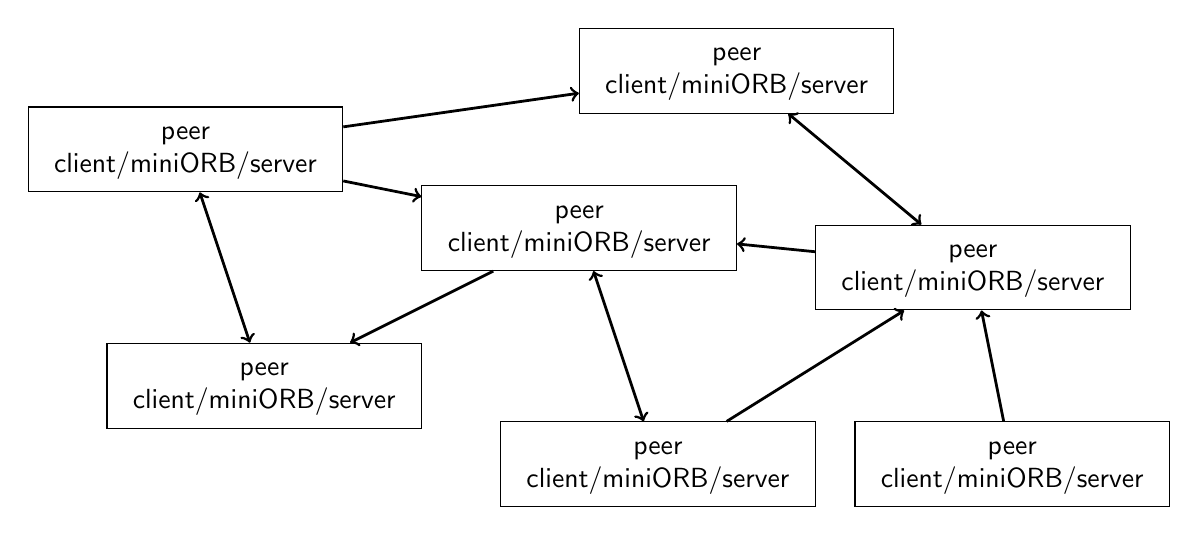
\begin{tikzpicture}[on grid, auto]
    \node[draw] (a) {\begin{tabular}{c}peer\\client/miniORB/server\end{tabular}};
    \node[draw, above right = 1cm and 7cm of a] (b) {\begin{tabular}{c}peer\\client/miniORB/server\end{tabular}};
    \node[draw, below right = 3cm and 1cm of a] (c) {\begin{tabular}{c}peer\\client/miniORB/server\end{tabular}};
    \node[draw, below right = 1cm and 5cm of a] (d) {\begin{tabular}{c}peer\\client/miniORB/server\end{tabular}};
    \node[draw, below right = 3cm and 1 cm of d] (e) {\begin{tabular}{c}peer\\client/miniORB/server\end{tabular}};
    \node[draw, below right = 0.5cm and 5cm of d] (f) {\begin{tabular}{c}peer\\client/miniORB/server\end{tabular}};
    \node[draw, below right = 2.5cm and 0.5cm of f] (g) {\begin{tabular}{c}peer\\client/miniORB/server\end{tabular}};

    \path[->, line width=1pt]  (a) edge node {} (b);
    \path[<->, line width=1pt] (a) edge node {} (c);
    \path[->, line width=1pt]  (a) edge node {} (d);
    \path[<->, line width=1pt] (d) edge node {} (e);
    \path[->, line width=1pt]  (d) edge node {} (c);
    \path[->, line width=1pt]  (f) edge node {} (d);
    \path[<->, line width=1pt] (f) edge node {} (b);
    \path[->, line width=1pt]  (e) edge node {} (f);
    \path[->, line width=1pt]  (g) edge node {} (f);
\end{tikzpicture}


\section{Gossip (epidemic algorithms)}

Gossip is the process by which an information will spread among
entities. Important technique to solve problem in dynamic large scale system
(scalable, simple, robust)

\begin{lstlisting}
push // telling something
pull // asking something
\end{lstlisting}

\subsection{Protocol Characterisitc}
\begin{itemize}
	\item Cyclic/periodic, pair-wise interaction between peers
	\item The amount of information exchanged is of (small)
	bounded size per cycle
	\item The state of each peer is bounded (small)
	\item During interaction between two peers, the state of one changes to
	reflect the state of the other.
	\item Selection of peer is random (full peer set or small set of neighbors)
	\item Reliable communication is not assumed
	\item Protocol cost is negligible
\end{itemize}

\subsection{Protocol Usage}
\begin{itemize}
	\item \textbf{Dissemenitation}: Spread information in a manner that produces
	bounded worst-case loads.
	\item \textbf{Repairing}: Anti-entropy protocols for repairing replicated data,
	which operate by comparing replicas and reconciling differences.
	\item \textbf{Membership}: pick a stable node from a given list then track
    processes \enquote{I've heard from recently} and $push$ them.
	\item \textbf{Aggregates}: Compute a network-wide aggregate. (e.g.\ number of nodes or
	computing average/max/min)
	\item \textbf{Network topology}: Protocols that arrange network topology
    (e.g.\ T-man algorithm for rings)
\end{itemize}

\subsection{Information dissemination}

\begin{itemize}
\item Start with one peer that wants to disseminate some message.
\item Then every peer does the following:

\begin{enumerate}
	\item Buffers every message (information unit) it receives up to a
	certain buffer capacity $b$
	\item Forwards that message a limited number of hops or time steps $t$
	\item Forwards the message each time to $f$ randomly selected set of
	processes (fan-out)
\end{enumerate}
\end{itemize}

\subsubsection{Infect-forever Model}
\begin{itemize}
	\item Fixed population of size $n$ (at round 1, one is infected)
	\item If infected, remains infected forever
	\item $Y_r$ is the number of individuals infected at round $r$
	\item $f$ is the number of individuals that infected ones try to infect
    \item $R$ is the number of round to infect all population
\end{itemize}

\begin{eqnarray*}
Y_r &\approx& \frac{1}{1+n \times e^{-f \times r}}\\
R &=& \log_{f+1}(n)+\frac{1}{f}\log(n)+O(1)\\
\end{eqnarray*}

\subsubsection{Infect-and-die model}

\begin{itemize}
\item Infectious process \enquote{remains infectious} for just one round
\item $\pi$ is the proportion of processes eventually contaminated
\item $R$ the number of round to infect entire system:
\end{itemize}

\begin{eqnarray*}
\pi &=& 1-e^{-\pi \times f}\\
R &=& \frac{\log(n)}{\log(\log(n))}+O(1)\\
\end{eqnarray*}

\subsubsection{Membership}

To ensure scalability, each process has a partial view (random sample of
node).

\begin{itemize}
	\item When a process forwards a message, it
	includes in this message a set of processes it knows.
	\item Hence, the process that receives the message can enhance the
	list of processes it knows by adding new processes.
\end{itemize}

\paragraph{Protocols requirement}

\begin{itemize}
\item \textbf{Uniformity}: all nodes play the same role
\item \textbf{Adaptivity under churn}: the parameters have to be tuned ($t$ and $f$)
\item \textbf{Bootstrapping}: how do nodes enter and leave, how to start
\end{itemize}


\subsubsection{Buffer Management}

Depending on broadcast rate, buffer capacity of processes may be
insufficient to ensure that every message is buffered long enough.

\paragraph{To counter that}
message are classified according to their
age (the number of processes the message went through) $\to$
Old messages are replaced.

\subsection{Small-world network}

There are different ways for a process to choose its infection target:

\begin{description}
	\item[Nearest-neighbor network] Targets are only neighbors (number of
	round is $\bigoh(n^{1/D})$ for a D-dimensional grid)
	\item[Random network] Target is random (number of rounds is
	$\bigoh(\log(n))$)
	\item[Small-world network] In between case (number of rounds
	is $\bigoh(\log(n))$)
\end{description}

\paragraph{Note:} Real world social network tends to be small-world networks.


\subsubsection{Properties}

Small-world network has both nearest neighbor connections as well as
long range connections (Node reachable with a small number of hops).

\paragraph{Properties}
\begin{itemize}
	\item Small average shortest path length (opposed to large path length
	in Neighbor graphs)
	\item A high clustering coefficient (opposed to low CC in Random graphs)
	\begin{description}
	\item[Clustering c\oe{}fficient] between 0 and 1 = Average of

        $$\forall_{p_i \in nodes} \frac{\sum { edge | \quad edge.start \in
            p_i.neighbors \quad AND \quad edge.end \in p_i.neighbors }}
            {p_i.nbrNeighbors (p_i.nbrNeighbors-1) /2)}$$

\end{description}
\end{itemize}

The clustering c\oe{}fficient (CC) measures degree of clustering. Count the
number of edges between neighboring nodes and divide by the maximum
possible for every node. The average of this number is the CC.

\subsection{Gossip Framework (Jelasity-Babaoglu)}
\begin{tabular}{m{0.5\linewidth}m{0.5\linewidth}}
\begin{lstlisting}[caption={Active thread}, mathescape]
do forever
    wait(T time units)
    q = SelectPeer()
    push S to q
    pull $S_q$ from q
    S = Update(S,$S_q$)
\end{lstlisting}
&
\begin{lstlisting}[caption={Passive thread}, mathescape]
do forever
    (p,$S_p$) = pull * from *
    push S to p
    S = Update(S,$S_p$)
\end{lstlisting}
\end{tabular}

To instantiate the framework, define
\begin{itemize}
	\item Local state $S$,
	\item Method \texttt{SelectPeer()} and \texttt{Update()}
	\item Style of interaction : \texttt{push, pull, push-pull}
\end{itemize}

\subsubsection{Aggregation}
The style of interaction is push-pull
\begin{itemize}
	\item $S$ is the current estimate of global aggregate
	\item \texttt{SelectPeer()}: Single random neighbor
	\item \texttt{Update()}: Numerical function defined according to desired global
	aggregate (arihtmetic/geometric mean,max,\ldots)
\end{itemize}

$$ \textrm{Converge factor} = \rho = \frac{E(\sigma^2_{i+1})}{E(\sigma^2_i)} \approx \frac{1}{2 \sqrt{e}} \approx 0.303 $$

\todo[inline]{Network size estimation}

\subsubsection{Topology Management}

Topology gradually appears as a result of a ranking function (can be provided
as an abstract service)

\begin{itemize}
\item Given a set of $N$ node (each node has a \texttt{view} of size $c$, \texttt{profile} is used
to calculate ranking)
\item Given a ranking function
    $$R: R(x, \{ y_1,\ldots,y_m \}) = {\textrm{all orderings of } \{y_1,\ldots,y_m\}} $$
\begin{itemize}
\item[$\to$] $R$ can be defined by a distance function $d(x,y)$
\end{itemize}
\end{itemize}

\paragraph{T-Man algorithm}

T-man is a general topology management service that converges quickly
(logarithmic) based on a gossip framework.

\begin{itemize}
    \item \texttt{InitialView()}: random sample of nodes
    \item \texttt{Merge($v_1, v_2$)}: $v_1 \cup v_2$
    \item \texttt{SelectPeer(v)}: rank current view $v$ according to $R$ and return
    random sample from first half
    \item \texttt{SelectView(b)}: rank $b$ according to $R$ and return first $c$ elements
\end{itemize}

\begin{lstlisting}[caption={Active thread}, mathescape]
view $\leftarrow$ initialView()
do at a random time once in each consecutive interval of T time units
    p $\leftarrow$ selectPeer()
    myDescriptor $\leftarrow$ (myAddress, myProfile)
    buffer $\leftarrow$ merge(view, {myDescriptor})
    send buffer to p
    receive view$_p$ from p
    buffer $\leftarrow$ merge(view$_p$, view)
    view $\leftarrow$ selectView(buffer)
\end{lstlisting}

\begin{lstlisting}[caption={Passive thread}, mathescape]
do forever
    (q, view$_q$) $\leftarrow$ waitMessage()
    myDescriptor $\leftarrow$ (myAddress, myProfile)
    buffer $\leftarrow$ merge(view, {myDescriptor})
    send buffer to q
    buffer $\leftarrow$ merge(view$_q$, view)
    view $\leftarrow$ selectView(buffer)
\end{lstlisting}

\paragraph{Convergence analysis}
There are two phases: \textbf{rapid convergence} phase followed by
\textbf{endgame} phase.

\begin{itemize}
\item After 1 cycle, view is closest $c$ out of $2c$
\item After $i$ cycles, view is closest $c$ out of $2^i c$
\end{itemize}

\subparagraph{Handling the endgame}

Near the end of the convergence, a few nodes are still left behind, there are
two improvements to manage them (depending on the actual topology):

\begin{itemize}
\item \textbf{Balancing}: during rapid convergence, receiving node refuses
contact if there are already too many
\item \textbf{Routing}: during endgame, instead of random selection of a
peer node, select closest one on the topology (with
exponentially decreasing probabilities)
\end{itemize}


\section{Bit torrent}

\paragraph{Problem}
\begin{itemize}
\item Large number of user $\bigoh(10^3)$
\item Fast as possible
\end{itemize}

\subsection{Naïve solution}
All client download from the server with the maximum
number of parallel client (depend of the available bandwith).

\paragraph{Problem}
It's really slow and to sequential ordering.
In addition, we don't use upload resources of clients.

\subsection{Pieces}

A file is sliced into a number of smaller transfer units called pieces of a
small predefined size.

\begin{itemize}
\item \textbf{Selecting the right peers}: From the point of view of one peer, selecting the
right peer to connect to can make a difference in the speed of downloading a file
\item \textbf{Selecting the right pieces}: Not only peer selection is important, piece
selection can affect the download time
\item[$\Rightarrow$] maximize the utilization of network resource of everybody
\end{itemize}

\subsubsection{Select peers and pieces}

\begin{itemize}
\item Global knowledge OR no global knowledge
\item[$\to$] In real P2P, the bandwith changes over time, peers come and go,
peers are selfish (Download file and run away)

\item[Solution]: random decision s.t
\begin{itemize}
\item Make sur that all peers have roughly the same number of links
\item A peer choose random piece from the peers he is connected
\end{itemize}
\end{itemize}

\subsection{Bittorent}

\subsubsection{Terminology}
\begin{description}
\item[Seeds]: machines that have a complete copy of the file. They are usually selfish and do not want to
wait after they get the file.

At least the first seed has to stay to serve
one complete copy of the file.

\item[Leechers]: Any peer who does not have a complete file
is called a leecher
\item[Tracker]: A peer that keeps track of who are the seeds and the leechers.
\item[Tracker.getPeers]: Give a subset of peers
\item[.torrent file/Meta-info File]: 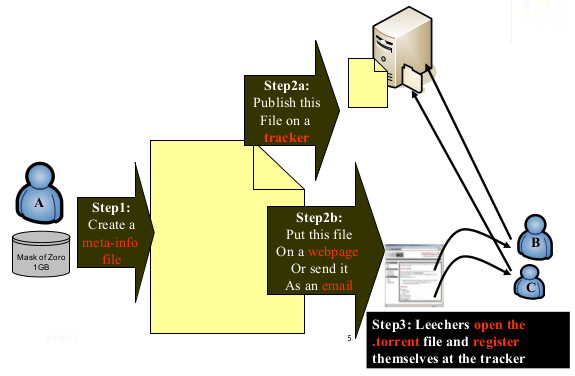
\includegraphics[width=7cm]{img/torrent.png}
\item[Handshaking]: Once a peer list is received, a handshake message
is sent to the all peers
\item[Exchanging bitfields] after handshaking with peers

\end{description}

\begin{figure}[!ht]
\centering
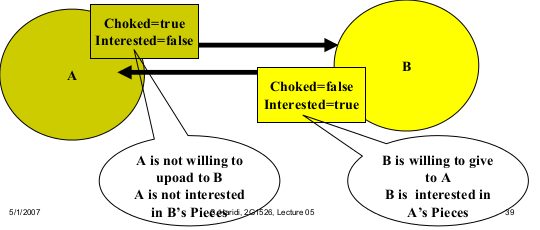
\includegraphics[width=9cm]{img/after.png}
\caption{After exchange}
\end{figure}
\FloatBarrier{}

%TODO Choking

\subsubsection{Piece selection}
\begin{itemize}
\item Rarest-first amoung your peers
\item Random-first piece to get first piece as fast as possible (only first few piece)
\item EndGame mode
\end{itemize}

\subsubsection{Peer selection}
\begin{enumerate}
\item Construction of the peer list by using the tracker
\item Unchoking (=Choice based on which peer can give me pieces faster)

\begin{itemize}
    \item A peer has a total of 80 connections, 40 initiated by
    him and 40 by others
    \item A peer unchokes only 4 peers simultaneously
    \item Decision about unchoking is reconsidered every ten
    seconds
    \begin{itemize}
        \item 3 peers are unchoked (given that they are interested)
        based on their upload rate to me
        \item Optimistically look for a fast guy randomly in the 40
        remaining connections
    \end{itemize}
\end{itemize}
\end{enumerate}


\section{Raft}

\begin{itemize}
    \item At any given time, each servier is EITHER:
        \begin{enumerate}
            \item Follower: completely passive
            \item Candidate: used to elect a new leader
            \item Leader
        \end{enumerate}
    \item Time divided into term (maintains current term value)
\end{itemize}

\subsection{Leader election}
\begin{enumerate}
    \item Increment current term
    \item Change to candidate state
    \item Vote for self
    \item Send request vote RPC to all other server
        \begin{itemize}
            \item Receive vote from majority $\Rightarrow$ leader
            \item Receive RPC from valid leader $\Rightarrow$ follower state
            \item Ellection timeout elapse $\Rightarrow$ new election
        \end{itemize}
\end{enumerate}

\subsection{Log replication}
Leader take commands from clients and replicates its log to other server.


\begin{thebibliography}{1}
\bibitem{icampus} http://www.icampus.uclouvain.be, {\em Icampus}
\end{thebibliography}

\end{document}
